%%% NOTE: I AM FIRST COMPILING MY TEX FILE IN VS Code; WILL TRANSFER CONTENT


% **Presentation Structure:**

% 1) Introduction: Problem Statement and Motivation
% 	- Why the problem is relevant; particular aspect we focus on (crossover disambiguation in sequential memory);
% 	- Goal
% 	- Quickly introduce the model we hope to implement; introduce idea of energetic approach
% 2) Lit Review
% 	* Important papers in the fields (including Krotov on DAM)
% 	* Clear Gap: no learning rules for disambiguation of crossover
% 3) Introduction of Model
% 	* Motivation for Kuramoto in a Hopfield Network (mention what we are hoping to observe: smoothness when retrieving, and mention importance to physical oscillator-based simulators)
% 	* Introduce basic learning rule (derived for Kuramoto from Krotov DAM) and algorithm for sequence retrieval; display graph for single sequence retrieval
% 	* Demonstrate the inability of the basic rule to resolve branching / crossover
% 	* Using argument on the innate symmetry of the energy landscape, introduce heterogeneous learning rules + motivation/reasoning
% 4) Experiment
% 	* Set up benchmarks
% 	* Table display of learning rules
% 	* Define experiment conditions; important global parameters
% 	* Experimental results, including superposition of learning rules
% 	* Display robustness, sweeping across different corruption ratios and N
% 	* Discussion: based on this talk about which learning rules perform better + limitations
% 5) Analytical Part (Jona)
% 	* Tensor notation: symmetric and asymmetric components
% 	* Scalability?
% 6) Conclusion + Applications
% 	* Quick notes on implementation into physical simulator and problems that this can solve (include those in Neurobiology?)


% UNSURE: in which order, benchmark first and then new learning rule or benchmark in section on experiment 

%%% NOTE: I AM FIRST COMPILING MY TEX FILE IN VS Code; WILL TRANSFER CONTENT

% =====================================================================
%  Crossover disambiguation in Kuramoto-coupled dense associative
%  sequential memory.
%
%  Deck structure (as built):
%    1  Introduction   -- crossover problem; Hebbian -> Krotov DAM ->
%                         Kuramoto sequence drive; asymmetric couplings
%                         give a Lyapunov function, NOT an energy
%    2  Literature     -- foundations; the open problem
%    3  Model          -- baseline rule + algorithm; its failure at a
%                         crossover; symmetry of the Lyapunov function;
%                         heterogeneous lag-context rules
%    4  Results        -- benchmarks, catalogue, conditions, crossover
%                         resolution, superposition, robustness,
%                         findings I (rules) and II (dynamics/scaling)
%    5  Analysis       -- tensor decomposition; scalability      [Jona]
%    6  Conclusions    -- main result; applications
%    7  Open questions -- physical implementation; decaying neurons;
%                         randomly generated sequences
%
%  Remaining \TODO{} placeholders mark numbers and figures to drop in
%  from the executed notebooks.
% =====================================================================

\documentclass[aspectratio=169]{beamer}

\usetheme{Madrid}
\usecolortheme{default}

\usepackage[utf8]{inputenc}
\usepackage{amsmath, amssymb}
\usepackage{booktabs}
\usepackage{graphicx}
\graphicspath{{../}{./}}
\usepackage{algorithm}
\usepackage{algpseudocode}
\usepackage{tikz}
\usetikzlibrary{arrows.meta, positioning}

% Convenience macros used throughout (edit to taste)
\newcommand{\xxi}{\xi}
\newcommand{\thetavar}{\theta}
\newcommand{\mvar}{m}
\newcommand{\TODO}[1]{{\color{red}\textbf{[TODO: #1]}}}
% Figure title: a short scientific label placed under each plot, above its caption.
\newcommand{\figtitle}[1]{\\[1mm]{\footnotesize\textbf{#1}}\\[1mm]}

\title[Kuramoto DAM: Crossover Disambiguation]{Context-informed Crossover Disambiguation in Kuramoto-Coupled\\ Dense Associative Sequential Memory}
\subtitle{Learning rules for resolving branch ambiguity in phase-oscillator sequence retrieval}
\author[D. Vorobiev \and J. N\"agerl]{Daniel Vorobiev \and Jona N\"agerl}
\institute{University of Cambridge}

\begin{document}

\begin{frame}
  \titlepage
\end{frame}

\begin{frame}{Outline}
  \tableofcontents
\end{frame}



% =====================================================================
\section[Introduction]{Introduction and Motivation}
% =====================================================================


% [EDITED per meeting: slide 3]
\begin{frame}{Sequential associative memory}
  \begin{columns}[T]
    \begin{column}{0.58\textwidth}
      \begin{itemize}\small
        \item \textbf{Associative Memory:} decoding sequences of stored patterns in a ``memory'' environment.
        \item Hopfield memories store \emph{static} attractors: inapplicable to sequential retrieval for a chain of transitions $\mu \to \mu+1$, where $\mu$ is a sequence member and encoded pattern. Unlike Hebbian learning, this calls for asymmetric network weights. 
        \item \textbf{Language:} inherent grammatical structures, language hierarchy.  
        \item \textbf{Reasoning:} by avoiding \textbf{hidden variables} or \textbf{high-dimensionality} in the network landscape, we hope to establish a framework for sequential reasoning.  
        \item \textbf{Neurobiology:} Hippocampal Sequence Replay, motor control.
      \end{itemize}
    \end{column}
        \begin{column}{0.42\textwidth}
        \centering
        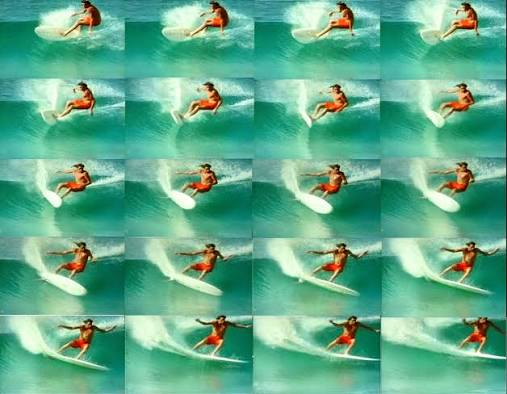
\includegraphics[width=\linewidth, height=0.5\textheight, keepaspectratio]{03_journal_club/figures/sequence.jpeg}
        \\[2mm]{\scriptsize Correlated successive patterns: constructive interference (following rules of causality and ``logic''), in contrast to uncorrelated patterns}
    \end{column}
  \end{columns}
\end{frame}


\begin{frame}{Scope of our investigation: context-dependent branching}
  \begin{columns}
    \begin{column}{0.55\textwidth}
      \begin{itemize}
        \item Assume two sequences share a contiguous run of patterns.
        \item At the shared/overlapping state the network configuration is
          \emph{identical} either way of branch; the sequential history  cannot encoded in the \textbf{microscopic state.}
        \item \textbf{History dependence:} introduce some macroscopic state variable to track pattern traversal history and inform branching choices.
      \end{itemize}
      \vspace{2mm}
      \centering\textbf{Can the coupling alone encode the route into $\xxi^0$?}
    \end{column}
    \begin{column}{0.35\textwidth}
      \centering
      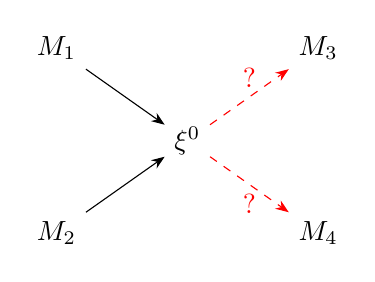
\begin{tikzpicture}[node distance=10mm, >=Stealth]
        \node (x0) {$\xxi^0$};
        \node (m1) [above left=6mm and 10mm of x0] {$M_1$};
        \node (m2) [below left=6mm and 10mm of x0] {$M_2$};
        \node (m3) [above right=6mm and 10mm of x0] {$M_3$};
        \node (m4) [below right=6mm and 10mm of x0] {$M_4$};
        \draw[->] (m1) -- (x0);
        \draw[->] (m2) -- (x0);
        \draw[->, dashed, red] (x0) -- (m3) node[midway, above] {?};
        \draw[->, dashed, red] (x0) -- (m4) node[midway, below] {?};
      \end{tikzpicture}\\[2mm]
      {\small Ambiguous sequence transitions from $\xxi^0$ shared by two sequences.\\
      Example: ``war \textbf{is} bad'' vs.\ ``peace \textbf{is} good'', shared element \textbf{``is''}.}
    \end{column}
  \end{columns}
\end{frame}

% [NEW per meeting: inserted after slide 4]
\begin{frame}{Encoding history: hidden variables vs.\ context drives}
  \begin{block}{Standard approach: hidden variables}
    Augment the state with hidden units $\Rightarrow$ higher-dimensional state space; sequences can be encoded as entire objects themselves.
  \end{block}
  \begin{block}{Our approach: context drives}
    No auxiliary units. The drive is gated by contextual (lagged) overlaps, and hence
    depends on the current position and history along the sequence. This allows to employ inherent properties of memory network, preserving the hierarchy between patterns and sequences.
  \end{block}
  \begin{itemize}
    \item \textbf{Information Trade-off:} the network has limited capacity for information; hence, there exists a risk of ``missing'' stored patterns upon sequence retrieval (as will be observed with reduced peak overlap values during the experimental stage).
  \end{itemize}
\end{frame}

% [EDITED per meeting: slide 5]
\begin{frame}{Objectives for Investigation}
  \begin{enumerate}
    \item A Kuramoto phase-oscillator DAM (Dense Associative Memory network) for encoding patterns into \emph{sequences}.
    \item A learning rule that resolves crossover from the coupling alone
      --- no external gating signal.
    \item \emph{When} is disambiguation possible at all, and how robust is
      it to corruption, network size and disorder?
    % [DROPPED per meeting] \item \TODO{one line: analytical / tensor contribution}
  \end{enumerate}
\end{frame}

% [EDITED per meeting: slide 6]
\begin{frame}{From Hebbian storage to Dense Associative Memory}
  \begin{columns}[T]
    \begin{column}{0.5\textwidth}
      \textbf{Hopfield (1982)} --- pairwise Hebbian
      $J_{ij} = \frac{1}{N}\sum_\mu \xxi_i^\mu \xxi_j^\mu$:
      \[
        E = -\tfrac{N}{2}\sum_\mu \bigl(\mvar^\mu\bigr)^2 ,\quad
        \mvar^\mu = \tfrac1N \sum_j \xxi^\mu_j s_j
      \]
      Crosstalk caps capacity at $\approx 0.14N$.
    \end{column}
    \begin{column}{0.5\textwidth}
      \textbf{Krotov--Hopfield DAM (2016)} --- sharpen the nonlinearity,
      i.e.\ higher-order interactions:
      \[
        E = -\sum_\mu F\bigl(\mvar^\mu\bigr), \quad F(x) = x^{\,d+1}
      \]
      Capacity $\mathcal{O}(N^{d})$; minima sharpen with $d$.
    \end{column}
  \end{columns}
  \vspace{1.5mm}
  \begin{block}{Resulting drive}
    Descending $E$ gives the \emph{pure-power} drive
    $\sum_\mu \xxi_i^\mu (\mvar^\mu)^{d}$. Every rule controls
    \emph{which} pattern each factor reads.
  \end{block}
  \begin{block}{Benefits}
    Increased storage capacity by reduction of crosstalk between stored patterns: essential for phase-sensitive retrieval of \textbf{sequences} of patterns. 
  \end{block}
\end{frame}

% [EDITED per meeting: slide 7; absorbs former slide 10]
\begin{frame}{Lifting the Krotov DAM to Kuramoto Couplings and Sequential Dynamics}
  \begin{enumerate}
    \item \textbf{Spins $\to$ phases:} $s_i = \cos\thetavar_i$, so
      $\dot\thetavar_i = -\partial_{\thetavar_i} E
       = \omega_i - \sin\thetavar_i \sum_\mu \xxi_i^{\mu}(\mvar^\mu)^d$.
    \item \textbf{Symmetric weights ($\mu \to \mu$):} true gradient flow; stored
      patterns are minima.
    \item \textbf{Asymmetric weights ($\mu \to \mu+1$):} \emph{essential for sequential dynamics}, drive the \emph{successor}
      (Sompolinsky--Kanter): stored patterns cease to be resting points and
      the state traverses the chain. At this stage, no explicit energy landscape exists and trivial gradient descend is inapplicable.
  \end{enumerate}
  \begin{block}{Why Kuramoto}
    \small
    \begin{itemize}
      \item \textbf{Physical systems.} Rules expressed purely as oscillator
        coupling are natively executable on analog and photonic hardware.
      \item \textbf{Continuous state variables.} Not restricted to binary
        patterns $\Rightarrow$ greater expressivity.
      \item \textbf{Smooth retrieval.} Continuous phases resolve the traversal of a
        crossover \emph{in time}, rather than as a discrete jump.
    \end{itemize}
  \end{block}
\end{frame}


% =====================================================================
\section[Model]{Retrieval Model and Learning Rules}
% =====================================================================

% [EDITED per meeting: slide 12]
\begin{frame}{What does sequence retrieval mean?}
  \begin{itemize}\small
    \item \textbf{Macroscopic variable, overlap $m^{\mu}$}, defines how ``close'' the current network state is to a stored pattern; this determines the retrieval dynamics. Below is the Krotov inspired \textbf{Baseline Forward:}
  \end{itemize}
  \[
    \dot\thetavar_i = \omega_i - \sin\thetavar_i \sum_\mu
      \xxi_i^{\mu+1}\,\bigl(\mvar_i^{\mu}\bigr)^{d}, \qquad
      \mvar_i^{\mu} = \frac{1}{N-1}\sum_{j\ne i}\xxi_j^{\mu}\cos\thetavar_j
  \]
  \begin{center}
    \small The network is in state $\boldsymbol{\thetavar} \in [0, 2\pi)^N$; each stored pattern
  $\boldsymbol{\xxi}^{\mu} \in \{-1,+1\}^N$ is an element of the sequence
  \[
    \mathcal{S} = \bigl(\boldsymbol{\xxi}^{0} \to \boldsymbol{\xxi}^{1} \to \cdots \to \boldsymbol{\xxi}^{P-1}\bigr).
  \]
    \[
  \{\boldsymbol{\xxi}^{\star}\} \subset \mathcal{S}^{A} \cap \mathcal{S}^{B}
    \]
  \end{center}
  \begin{algorithm}[H]
    \small
    \begin{algorithmic}[1]
      \State cue $\thetavar(0) \gets$ (possibly corrupted) $\xxi^{0}$
      \For{each step}
        \State $\mvar^\mu_i$ for all $\mu$; \; $V_i = \sum_\mu \xxi_i^{\mu+1}(\mvar_i^\mu)^d$
        \State $\thetavar_i \mathrel{+}= dt\,(\omega_i - \sin\thetavar_i V_i)$ \; ($+$ noise)
      \EndFor
      \State decode the sequence from overlap peaks
    \end{algorithmic}
  \end{algorithm}
\end{frame}

% [EDITED per meeting: slide 13]
\begin{frame}{Sequential Memory Retrieval: Overlap Evolution under Baseline Rule}
  \centering
  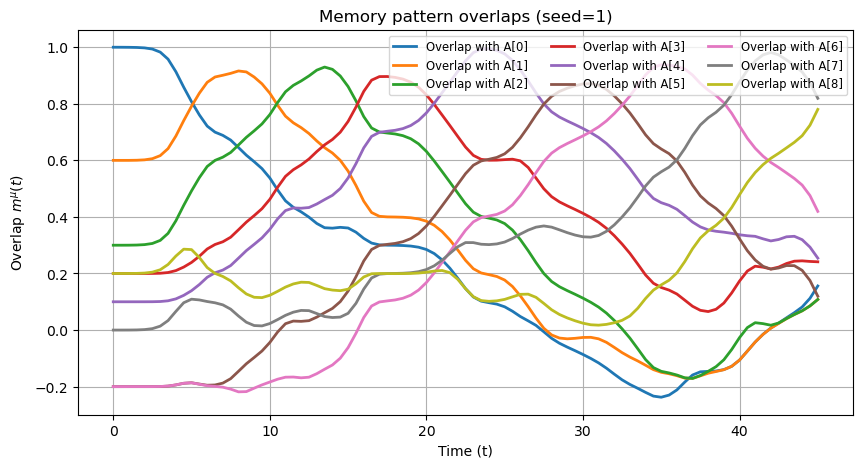
\includegraphics[height=0.68\textheight,width=\textwidth,keepaspectratio]{03_journal_club/figures/s_seq.png}
  \figtitle{$\mvar^\mu(t)$ for single-sequence retrieval under the baseline (\texttt{forward}) rule}, N=40.

\end{frame}

% [REDONE per meeting: former slide 9, moved after slide 13; old content kept after \end{document}]
\begin{frame}{Why should the Krotov DAM fail at branching?}
  \begin{itemize}
    \item \textbf{Microscopic:} the dynamics are deterministic in the phases $\thetavar$.
    \item \textbf{Macroscopic:} distinct trajectories can nevertheless end up at the
      same overlap --- the macroscopic order parameter (or partial overlaps). 
    \item The baseline forward rule \textbf{only carries information about the current and one subsequent states}; no information regarding \textbf{context}, i.e. previous patterns, is being accessed.
  \end{itemize}
\end{frame}

% [EDITED per meeting: slide 14]
\begin{frame}{Baseline rule at a crossover}
  \centering
  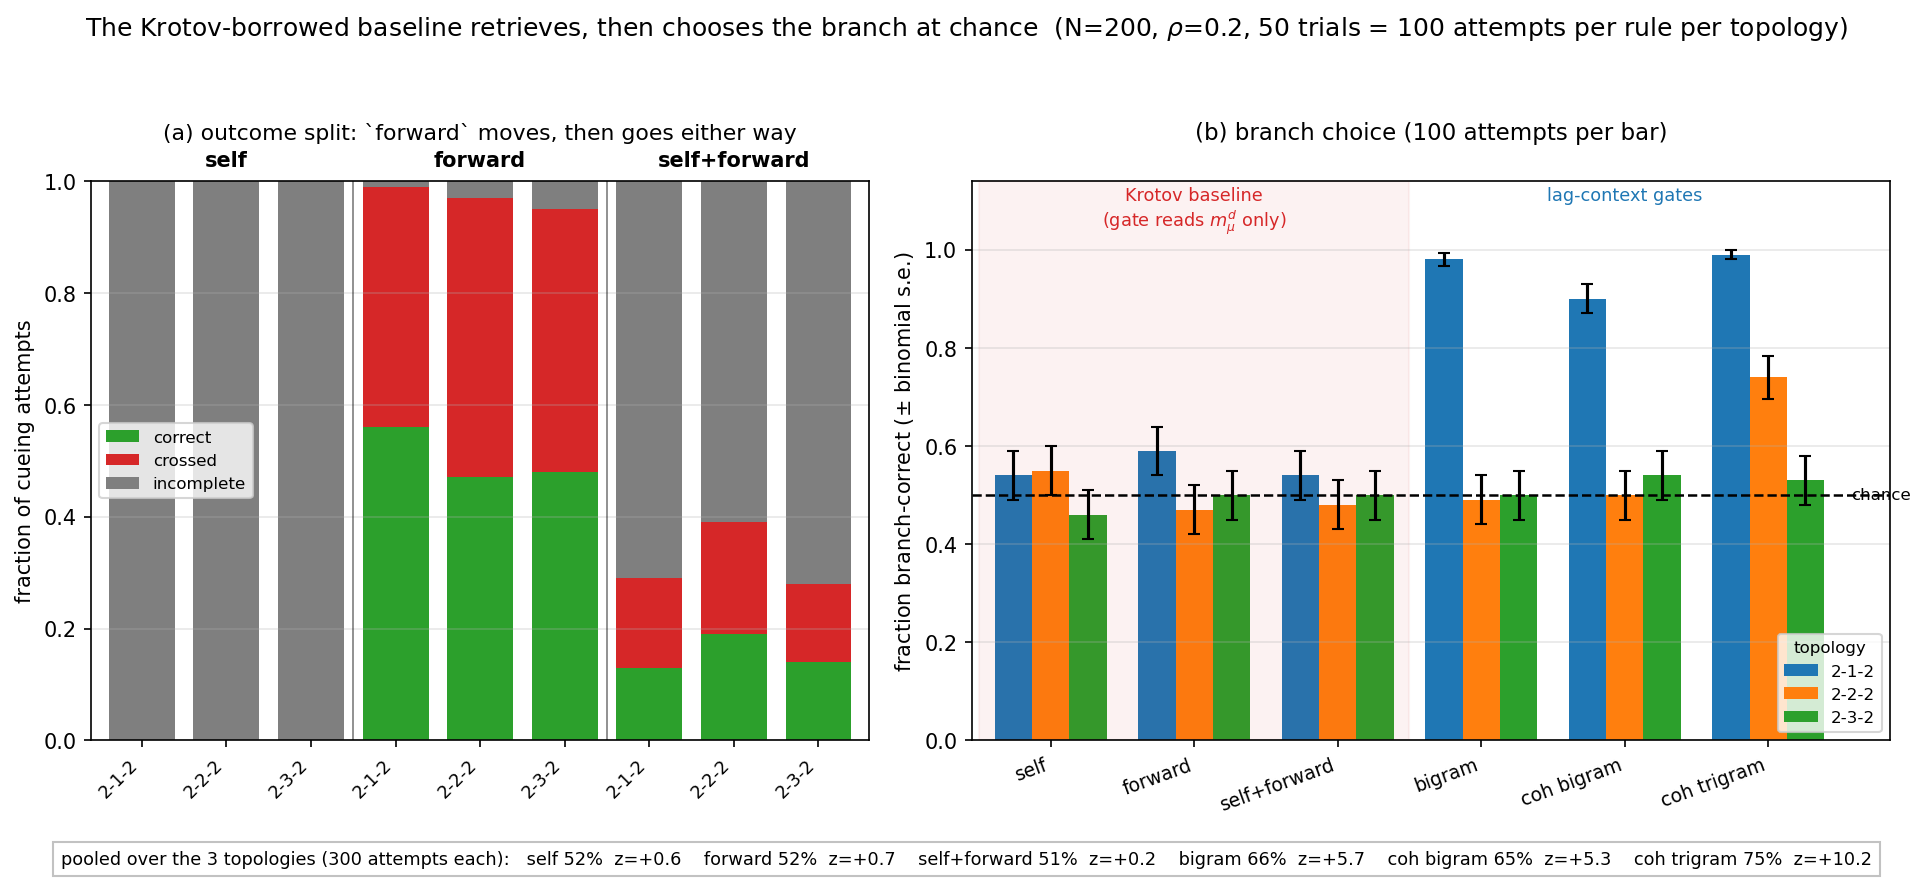
\includegraphics[height=0.56\textheight,width=0.8\textwidth,keepaspectratio]{03_journal_club/figures/fig12_baseline_chance.png}
  \figtitle{Branch overlaps out of the shared state at a crossover, baseline (\texttt{forward}) rule}
  {\small Both continuations rise together out of the shared state.
  Branch choice at chance.}
\end{frame}

% [EDITED per meeting: slide 16; former slide 21 follows]
\begin{frame}{Learning rules to resolve crossover}
  \[
    \dot\thetavar_i = \omega_i - \sin\thetavar_i \sum_{\mu}\sum_{\text{terms}}
      w \;\xxi_i^{\mu+s} \prod_{l \in \text{lags}} \mvar_i^{\mu - l}
  \]
  \begin{itemize}
    \item A rule is a \emph{table of terms}: target offset $s$, $d$ source
      lags, weight $w$. Lags $(0,0,0)$ recovers the forward rule.
    \item Different lags in one term $\Rightarrow$ the gate encodes
      \emph{which branch} produced the current state.
    \item \textbf{Intuition:} superposition of references ("lags") to previous network states and patterns, \textbf{for context}.
  \end{itemize}
\end{frame}

% [MOVED per meeting: former slide 21]
\begin{frame}{Catalogue of learning rules}
  \centering
  \small
  \begin{tabular}{lll}
    \toprule
    Rule & Gate at pattern $\mu$ & Reach \\
    \midrule
    \texttt{self} & $\xxi^\mu \mvar_\mu^3$ & 0 (control) \\
    \texttt{forward} (baseline) & $\xxi^{\mu+1} \mvar_\mu^3$ & 0 \\
    \texttt{skip-two} & $\xxi^{\mu+2} \mvar_\mu^3$ & 0 \\
    \texttt{bigram} & $\xxi^{\mu+1} \mvar_\mu |\mvar_{\mu-1}|^2$ & 1 \\
    \texttt{multilag} & $\xxi^{\mu+1} \mvar_\mu \sum_k w_k |\mvar_{\mu-k}|^2$ & $\le K$ \\
    \texttt{coh bigram} & $\xxi^{\mu+1} \mvar_\mu^2 \mvar_{\mu-1}$ & 1 \\
    \texttt{coh trigram} & $\xxi^{\mu+1} \mvar_\mu \mvar_{\mu-1} \mvar_{\mu-2}$ & 2 \\
    \bottomrule
  \end{tabular}
  \\[3mm]
  {\small Reach $\ge L$ is the entry requirement for accessing \emph{any} unshared
  information. Clearing it does not guarantee the rule can use it.}
\end{frame}


% =====================================================================
\section[Results]{Numerical Experiments and Results}
% =====================================================================
%  Structure mirrors results_summary.ipynb:
%    1 why anything moves      2 why branching is hard
%    3 metrics / topologies / statistics
%    4 robustness              5 appendix
%  Figures: presentation/figures/, generated by that notebook.
% =====================================================================


\begin{frame}{How the experiments are organised}
  \begin{enumerate}
    \item \textbf{Why anything moves.} $\omega \equiv 0$ is an exact fixed point;
      the natural frequency is what starts the cascade, and how much of it matters.
    \item \textbf{Why branching is hard.} A shared run is bit-identical between
      branches; the gate must \textbf{reach past it} for {context}.
    \item \textbf{Metrics, topologies, statistics.} Four crossover metrics, four
      geometries, $100$-instance seed sweeps with spread.
    \item \textbf{Robustness.} Network size, corruption ratio, and two knobs on the drive.
    \item \textbf{Appendix.} Random patterns; settle vs.\ loop.
  \end{enumerate}
  \vspace{2mm}
  {\small Every number below is reproduced by \texttt{results\_summary.ipynb}.}
\end{frame}

\begin{frame}{Sequence construction: smooth corruption chains}
  \begin{columns}[T]
    \begin{column}{0.56\textwidth}
      \begin{itemize}
        \item $\xxi^{1}$ uniform on $\{0,\pi\}^N$; then
          $\xxi^{k+1} = \mathrm{corrupt}(\xxi^{k},\rho)$: $\lfloor \rho N \rfloor$ sites
          drawn without replacement, $\varphi \to \pi - \varphi$.
        \item Consecutive overlap is therefore fixed by construction:
          \[
            \tfrac1N \textstyle\sum_i \xxi^{k}_i \xxi^{k+1}_i = 1 - 2\rho,
            \qquad d(\xxi^k,\xxi^{k+1}) = 2\rho .
          \]
        \item The patterns form a \emph{chain}: neighbours stay inside each
          other's basin, which is what lets the cascade hop at all.
        \item Lagged overlaps decay geometrically,
          $\mvar_{\mu-\ell} \sim (1-2\rho)^{\ell}$: hence the gain filter's
          $(1-2\rho)^{-\sum\text{lags}}$.
      \end{itemize}
    \end{column}
    \begin{column}{0.44\textwidth}
      \centering
      \begin{tikzpicture}[node distance=6mm, >=Stealth, font=\scriptsize]
        \node (a1) {$\xxi^{A,1}$};
        \node (a2) [right=of a1] {$\xxi^{A,2}$};
        \node (s)  [right=of a2] {$\boxed{\xxi^{\star}}$};
        \node (a4) [above right=4mm and 7mm of s] {$\xxi^{A,4}$};
        \node (b4) [below right=4mm and 7mm of s] {$\xxi^{B,4}$};
        \node (b2) [below left=11mm and 0mm of a2] {$\xxi^{B,2}$};
        \node (b1) [left=of b2] {$\xxi^{B,1}$};
        \draw[->] (a1) -- (a2); \draw[->] (a2) -- (s);
        \draw[->] (b1) -- (b2); \draw[->] (b2) -- (s);
        \draw[->] (s) -- (a4); \draw[->] (s) -- (b4);
      \end{tikzpicture}
      \\[2mm]
      {\scriptsize Shared run generated \emph{once} and reused by both branches: those
      overlaps are bit-identical, so the ambiguity is exact. Each branch is an
      independent corruption chain off the run.}
      \\[2mm]
      {\scriptsize Uncorrelated patterns score $0\%$ for every rule --- nothing
      retrieves without the chain.}
    \end{column}
  \end{columns}
\end{frame}


\begin{frame}{Benchmarks}
  \centering
  \small
  \begin{tabular}{llccl}
    \toprule
    Tag & Geometry & $P$ & Shared run $L$ & Reach needed \\
    \midrule
    \texttt{2-1-2} & one shared pattern   & 5 & 1 & 1 \\
    \texttt{2-2-2} & shared segment       & 6 & 2 & 2 \\
    \texttt{2-3-2} & failure case         & 7 & 3 & 3 (beyond catalogue) \\
    \bottomrule
  \end{tabular}
  \\[3mm]
  \begin{itemize}
    \item \textbf{Scoring:} every \emph{unshared} pattern of the cued branch
      decoded, in order. Shared positions carry no rule information and are
      excluded.
    \item \textbf{Branch diagnostic:} correct vs.\ incorrect drive at the
      exit; separates incorrect selection from correct selection without
      lock-on.
  \end{itemize}
\end{frame}

\begin{frame}{Metrics used throughout}
  \centering\scriptsize
  \begin{tabular}{llp{5.9cm}l}
    \toprule
    & metric & definition & chance / floor \\
    \midrule
    \multicolumn{4}{l}{\textbf{Crossover} --- \texttt{2-1-2}, \texttt{2-2-2}, \texttt{2-3-2}; shared positions excluded} \\
    \midrule
    1 & \texttt{correct}        & every unshared pattern of the cued branch decoded \emph{in order}, before the other branch appears & --- \\
      & \texttt{crossed}        & the other branch appears first & --- \\
      & \texttt{incomplete}     & the run ended before the branch resolved & --- \\
    2 & overlap quality         & mean peak overlap of those patterns, successful attempts only, with spread & --- \\
    3 & \textbf{branch-correct} & did the trajectory favour the cued continuation? & $0.5$ \\
    4 & margin                  & signed gap between the cued and the other continuation's peak overlap & $0$ \\
    \midrule
    \multicolumn{4}{l}{\textbf{Single chain} --- $P = 10$, no branch} \\
    \midrule
    5 & retrieval fraction      & how much \emph{of a} sequence came back; partial credit on a strict prefix & $1/P = 0.10$ \\
    6 & strict rate             & how many \emph{of the} sequences came back whole & --- \\
    \bottomrule
  \end{tabular}
  \\[2mm]
  \begin{itemize}\scriptsize
    \item A pattern counts as decoded at overlap $\ge$ \texttt{tolerance} $= 0.5$.
    \item \textbf{Metric 3 isolates the decision}; metric 1 bundles it with completion,
      $\text{correct} \approx \text{branch-correct} \times (1 - \text{incomplete})$.
    \item \texttt{self} is the control in both regimes, and \texttt{forward} the baseline at a crossover.
  \end{itemize}
\end{frame}

\begin{frame}{Global parameters}
  \centering
  \footnotesize
  \begin{tabular}{llll}
    \toprule
    Symbol & Value & Symbol & Value \\
    \midrule
    $N$             & $200$ crossover; $100$ single (swept) & $dt$          & $0.05$ \\
    $P$             & $5,6,7$ crossover; $10$ single      & $T$             & $80$ crossover; $180$ single \\
    $d$             & $3$                                 & integrator      & Euler / Euler--Maruyama \\
    $\rho$          & $0.2$ (sweep $0.05$--$0.35$)        & early stop      & $\max_i|\dot\thetavar_i| < 10^{-6}$, $10$ steps \\
    $\mu_\omega$    & $0$                                 & tolerance       & $0.5$ overlap to decode a pattern \\
    $\sigma_\omega$ & $0.3$                               & decoder margin  & $0.01$ crossover; $10^{-3}$ single \\
    phase noise     & $0.01$ (inert: ODE mode)            & dwell           & $20$ per transition \\
    trials          & $20 \times 2$ cues; $100$ seed sweep & seeds          & pool of $10^4$ \\
    \bottomrule
  \end{tabular}
  \\[3mm]
  \begin{itemize}
    \item $\omega \neq 0$ is load-bearing --- see next slide.
    \item Raw and gain-corrected catalogues are run at every operating point;
      the gain is rebuilt at each $\rho$ of a sweep.
    \item \textbf{Two base sizes.} Branch choice saturates at $N = 200$, so the crossover
      experiments run there. The single-chain sweeps keep $N = 100$ as their base and sweep
      $N$ explicitly --- that sweep \emph{is} the experiment.
    \item \textbf{Caveat:} every network uses \texttt{seed=10}, so one $\omega$
      draw is reused throughout. On the $\omega$ axis every result is $n = 1$.
  \end{itemize}
\end{frame}

% ---------------------------------------------------------------- 1
\begin{frame}{1. Why anything moves: the natural frequency}
  \centering
  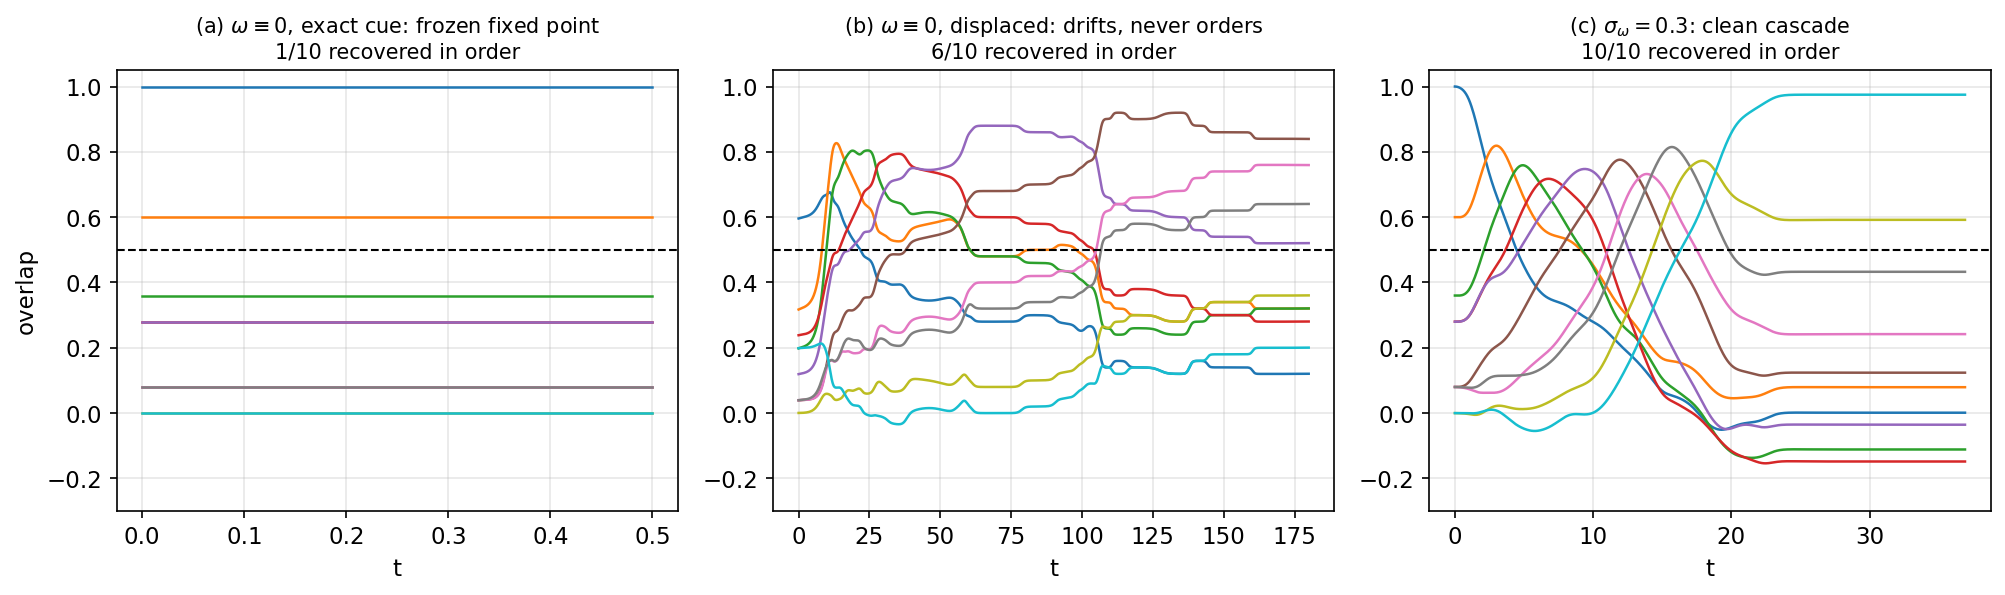
\includegraphics[width=\textwidth,height=0.45\textheight,keepaspectratio]{figures/fig01_stall.png}
  \figtitle{Retrieval at $\omega \equiv 0$ from an exact cue (a) and a displaced cue (b), against $\omega = 0.3$ (c)}
  {\scriptsize Note the differing time axes: (a) exits at the stationary early-stop within a
  few steps.}
  \begin{itemize}\small
    \item At an exact cue every $\thetavar_i \in \{0,\pi\}$, so $\sin\thetavar_i = 0$ and the
      coupling $-\sin\thetavar_i V_i$ vanishes \emph{identically}.
    \item \textbf{(b)} displaced start (flips \emph{plus} angular jitter, 
      off-lattice). No reliable cascade -- most likely an issue with time-resolution during dynamics integration.
    \item \textbf{(c)} $\omega = 0.05$: a clean cascade, each pattern peaking in turn and
      the full chain recovered in order.
  \end{itemize}
\end{frame}

\begin{frame}{1. How much frequency? The usable band}
  \centering
  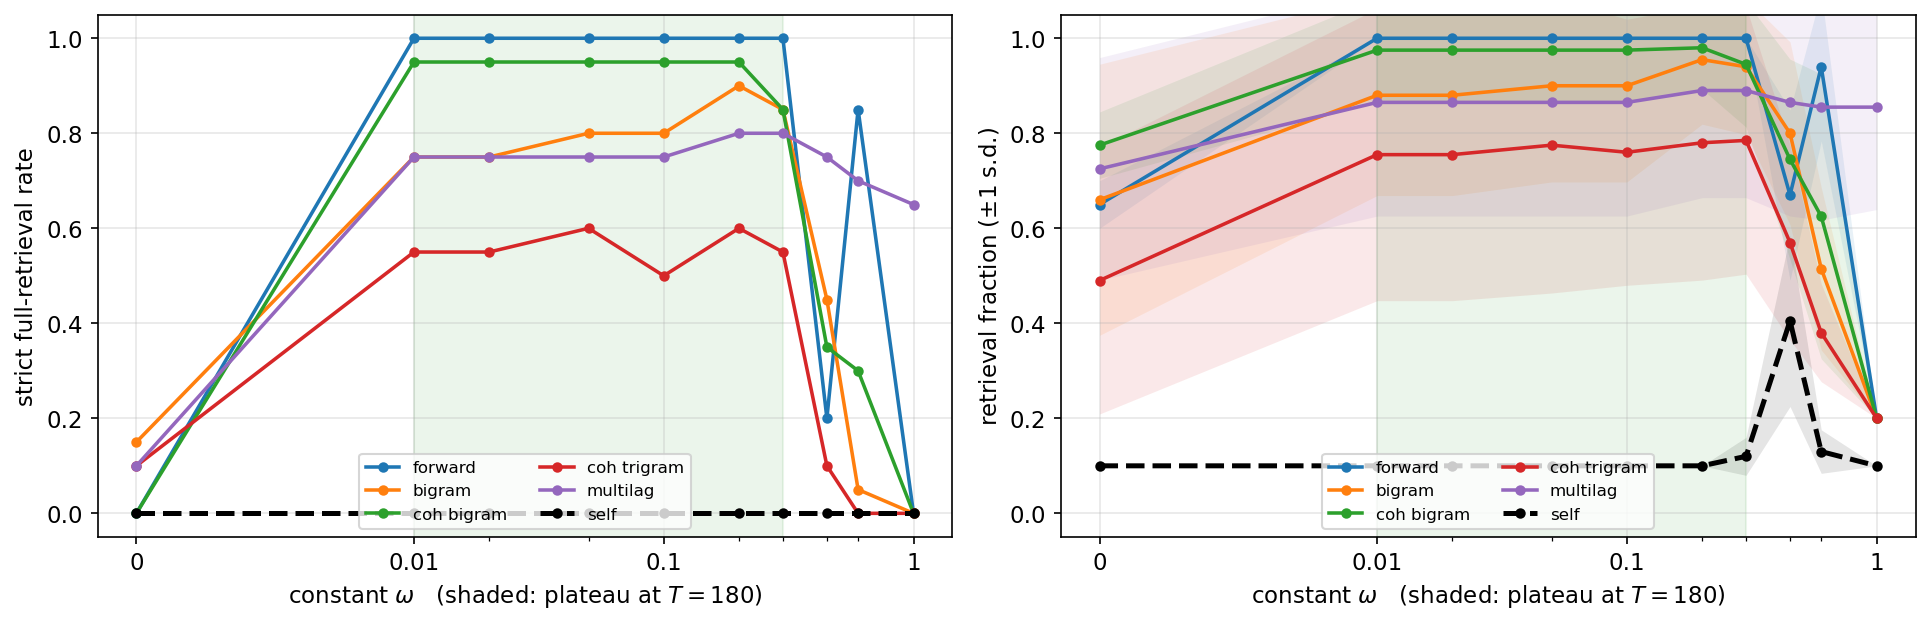
\includegraphics[width=\textwidth,height=0.43\textheight,keepaspectratio]{figures/fig02_omega_band.png}
  \figtitle{Retrieval fraction against $\omega$ at $T = 54$ and $T = 180$, by learning rule}
  \begin{itemize}\small
    \item $\omega = 0$ is \textbf{singular}: at an exact cue it is a fixed point, and any
      $\varepsilon > 0$ already sits in a different regime.
    \item A rotating frame \textbf{cannot} absorb a uniform $\omega$ here --- the drive is
      anchored to the absolute $\{0,\pi\}$ lattice, so the frame shift survives in the dynamics.
    \item At high $\omega$ ($\approx 1$) the drive is overwhelmed by the natural frequency: the
      overlaps never peak and noise is dominant. The usable band is $\sigma_\omega \in [0.1,0.5]$.
  \end{itemize}
\end{frame}

% ---------------------------------------------------------------- 2
% [EDITED per meeting: slide 25]


% ---------------------------------------------------------------- 3
% [EDITED per meeting: slide 26]
\begin{frame}{2. The four crossover metrics for branching disambiguation}
  \centering\footnotesize
  \begin{tabular}{clp{7.2cm}}
    \toprule
    \# & metric & definition \\
    \midrule
    1 & outcome & \texttt{correct} $=$ every unshared pattern of the cued branch, \emph{in
        order}, before the other appears; \texttt{crossed} $=$ wrong branch first;
        \texttt{incomplete} $=$ ran out \\
    2 & overlap quality & mean peak overlap of those patterns, over successful attempts only,
        with spread \\
    3 & \textbf{branch-correct} & did the trajectory favour the right continuation?
        Chance $= 0.5$ \\
    4 & margin & signed gap between the cued and the other continuation's peak overlap \\
    \bottomrule
  \end{tabular}
  \\[3mm]
  \begin{itemize}\small
    \item \textbf{Metric 3 is the one that matters}: it isolates the \emph{decision}.
      Metric 1 bundles it with completion, and empirically
      $\text{correct} \approx \text{branch-correct} \times (1 - \text{incomplete})$
      to within $\sim 6\%$ --- a low \texttt{correct} is always two failures multiplying.
    \item \texttt{correct} is also a strict AND over $\sim 4$ positions: $0.87$ per position
      reads as $57\%$. Shared positions are excluded throughout.
    
  \end{itemize}
\end{frame}

\begin{frame}{2. Overlap runs averaged across trials: an illustration}
  \centering
  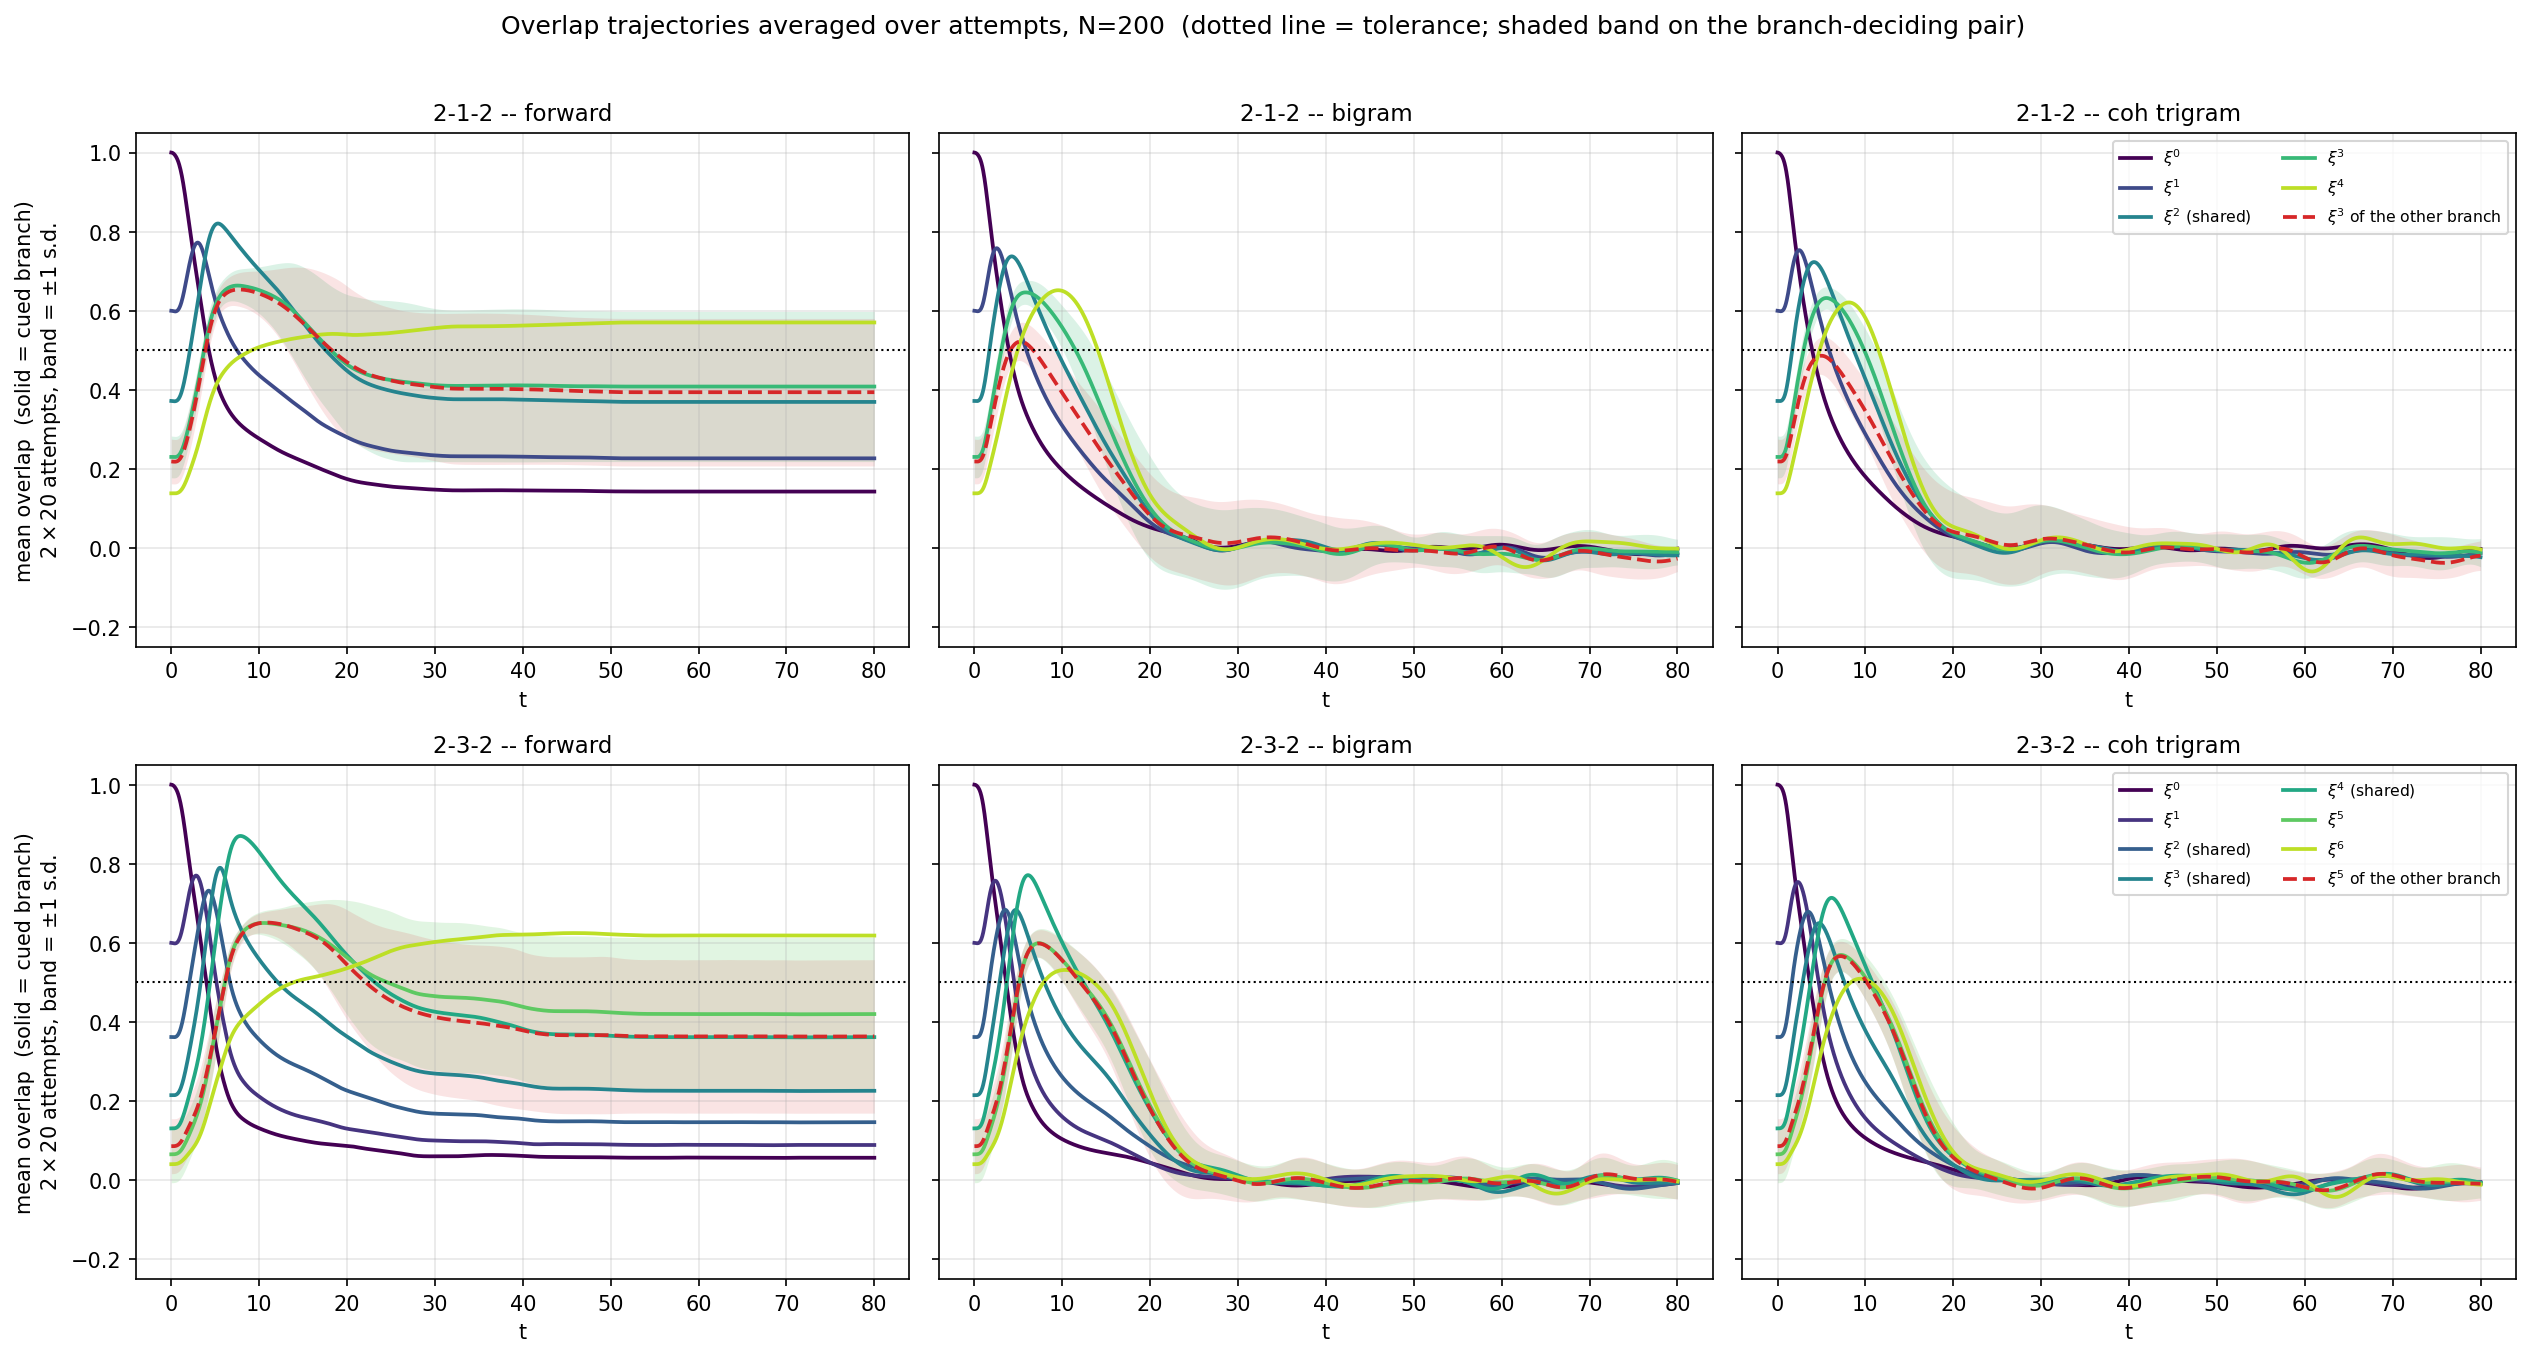
\includegraphics[width=\textwidth,height=0.66\textheight,keepaspectratio]{03_journal_club/figures/fig11_mean_overlap_traces.png}
  \figtitle{Branch overlaps $\mvar(t)$ averaged over all cueing attempts, by rule (columns) and geometry (rows)}
  {\small The decay for bigram and trigram learning rules reflects loss of information when referencing lags.}
\end{frame}



% [MOVED per meeting: former slide 29, moved to position 27]
\begin{frame}{3. One hundred instances, with statistics}
  \centering
  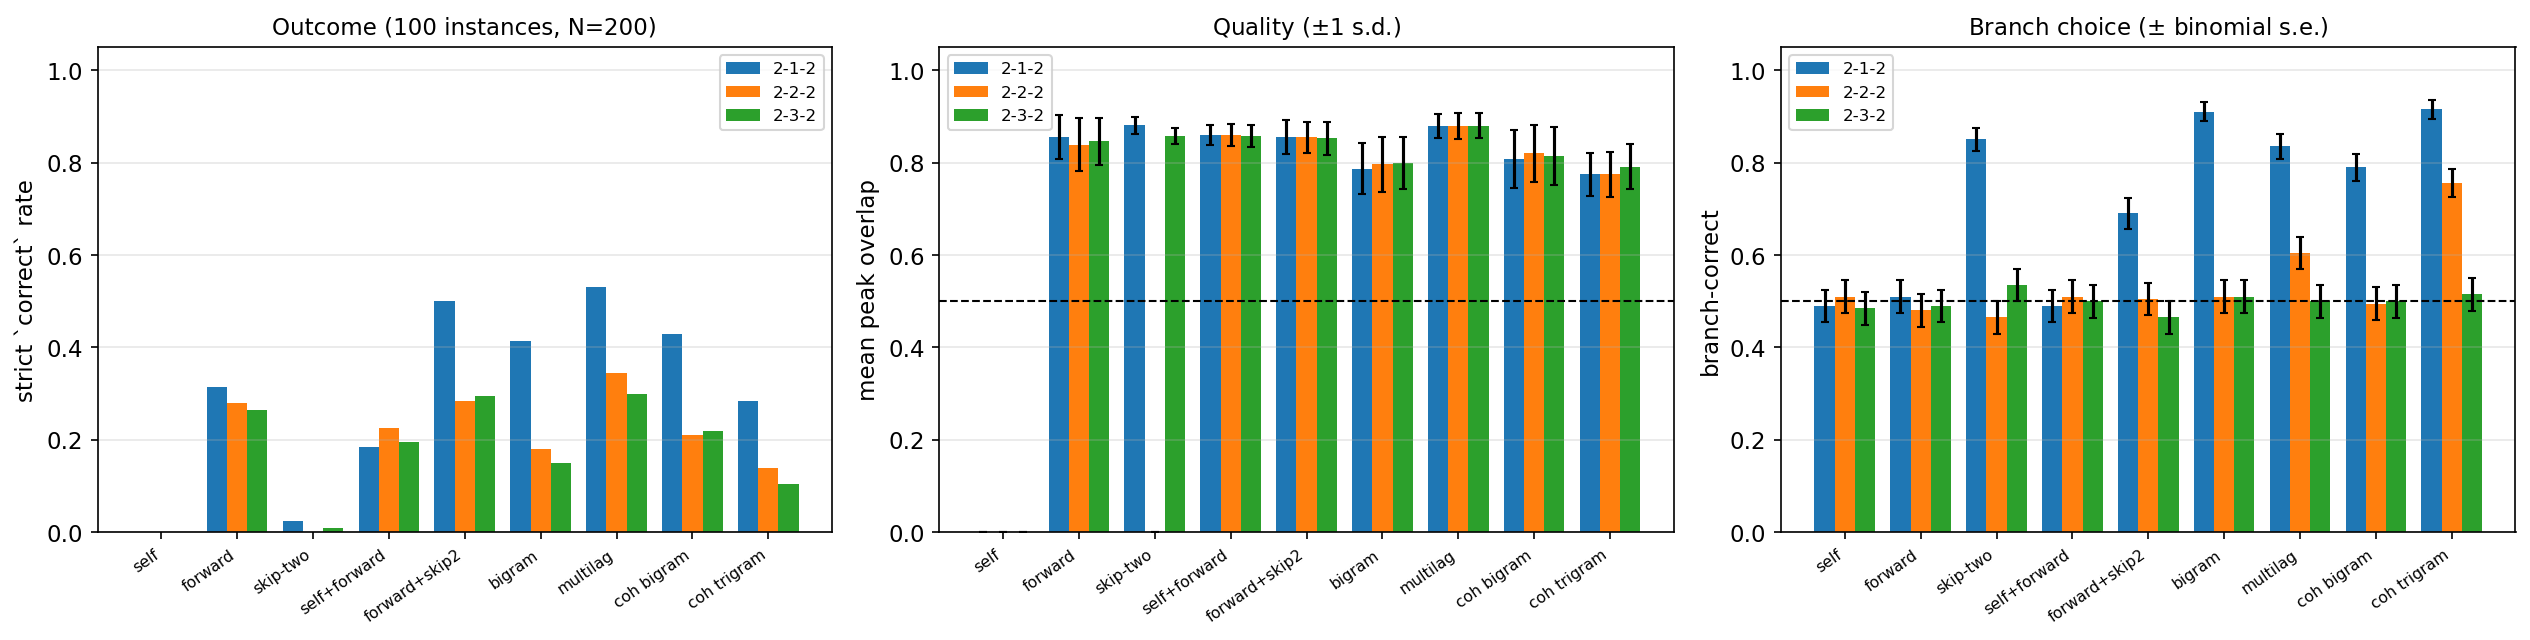
\includegraphics[width=\textwidth,height=0.56\textheight,keepaspectratio]{figures/fig06_seed_sweep.png}
  \figtitle{Retrieval quality and branch choice over $100$ crossover instances per rule}
  {\scriptsize $100$ crossover instances per rule, corruption rate drawn per trial from
  $U[0.12,0.28]$ so each rule faces a range of difficulties; identical instances across rules.
  Error bars: $1$ s.d.\ (quality), binomial s.e.\ (branch choice).}
\end{frame}

% [EDITED per meeting: slide 27]
\begin{frame}{3. Benchmark across geometries}
  \centering
  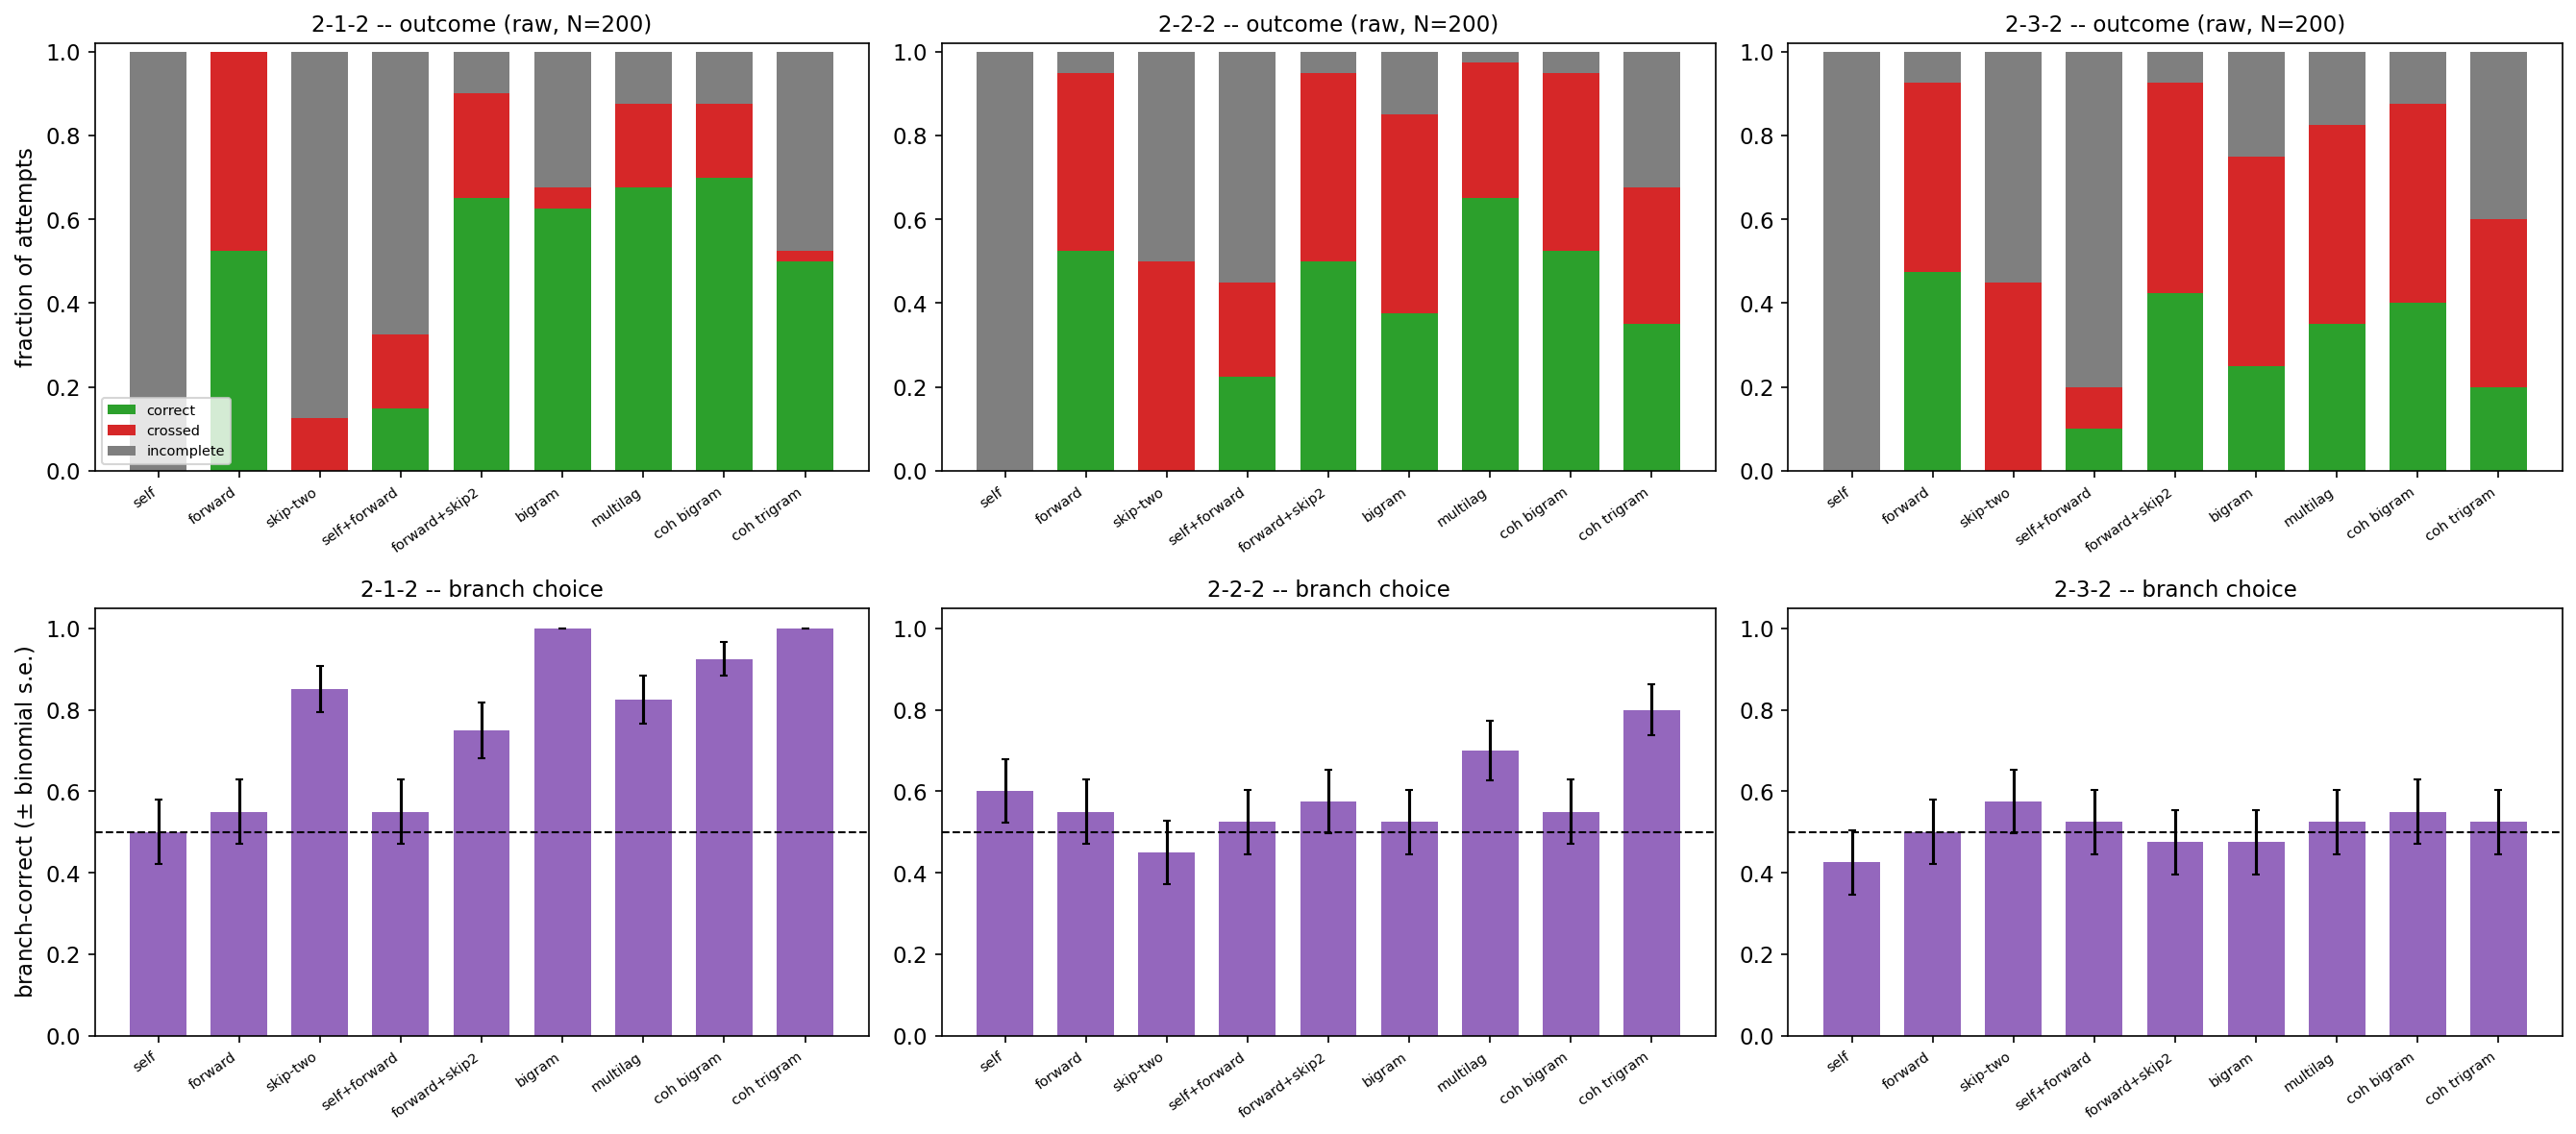
\includegraphics[width=\textwidth,height=0.58\textheight,keepaspectratio]{figures/fig04_benchmark.png}
  \figtitle{Outcome split and branch-correct rate by rule across crossover geometries}
  {\scriptsize Top: outcome split. Bottom: branch choice, $\pm$ binomial standard error
  $\sqrt{p(1-p)/n}$. Dashed line $=$ chance.}\\[1mm]

\end{frame}

\begin{frame}{3. Branch choice improves with network size}
  \centering
  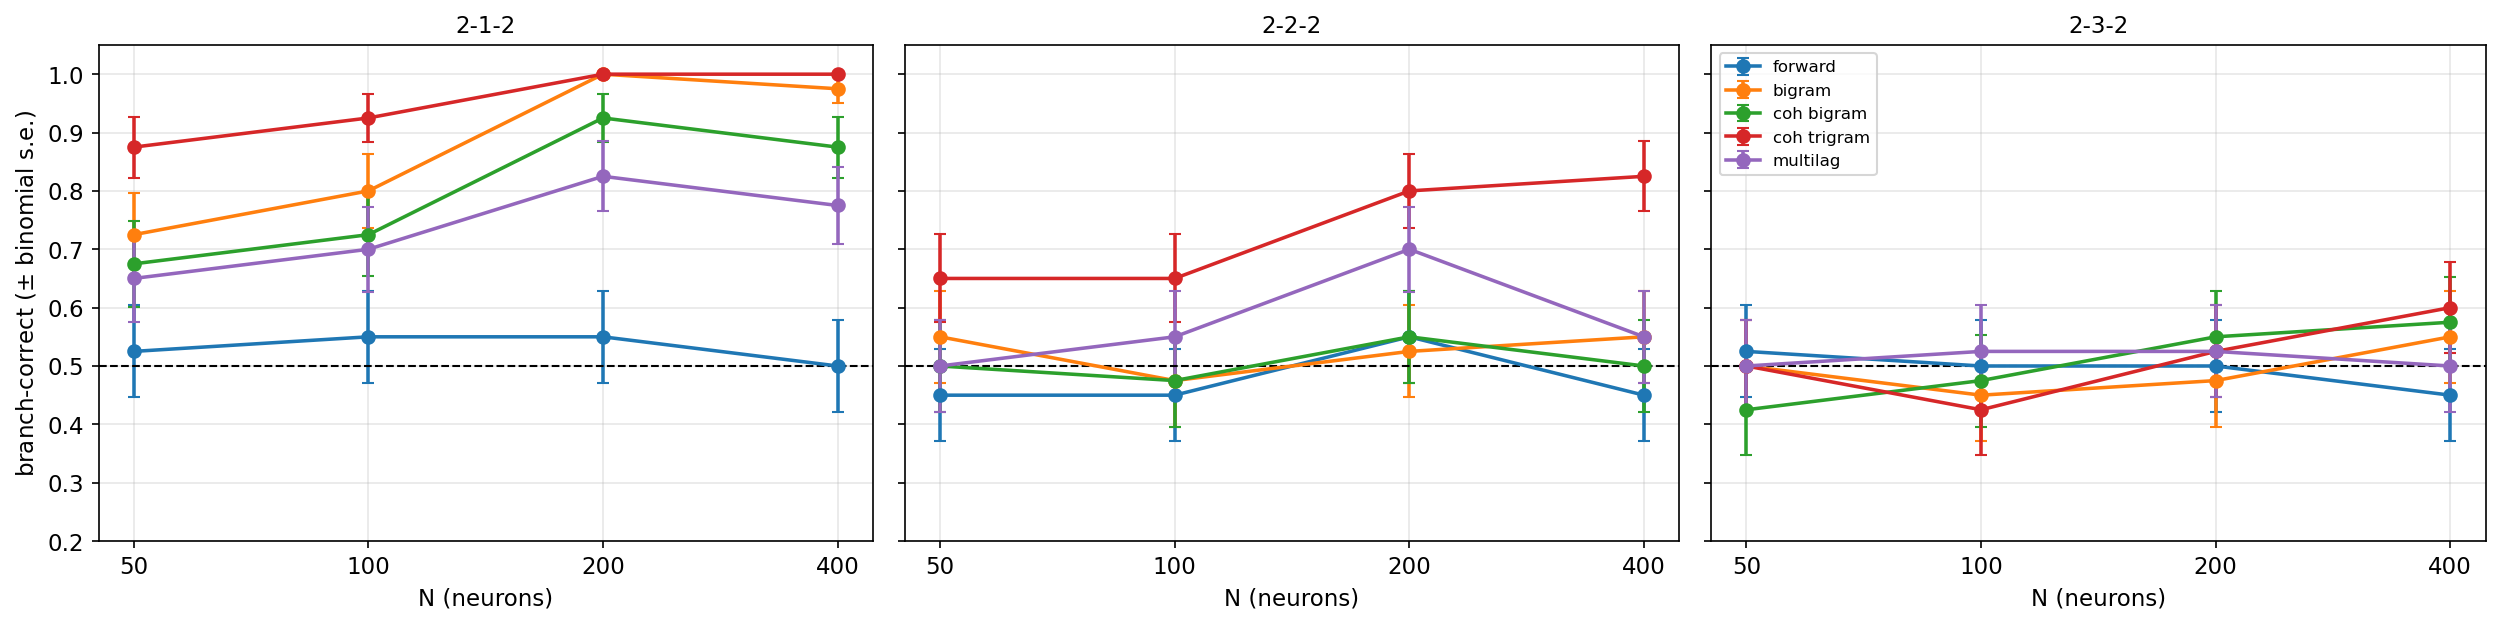
\includegraphics[width=0.96\textwidth,height=0.52\textheight,keepaspectratio]{figures/fig05_branch_vs_N.png}
  \figtitle{Branch-correct rate against network size $N$ on \texttt{2-1-2}}
  \begin{itemize}
    \item \textbf{The control works:} \texttt{forward} stays at chance
      ($55 \to 55 \to 50\%$). Network size does not manufacture branch information
      where the gate has none.
    \item \textbf{Across $N$, read branch-correct}: at fixed duration
      \texttt{incomplete} rises with $N$ (a larger network needs longer to traverse), so
      \texttt{correct} understates the gain.
  \end{itemize}
\end{frame}

% [EDITED per meeting: slide 30 -- lighter]
\begin{frame}{3. Which rule performs better}
  \centering\footnotesize
  \begin{tabular}{llp{6.6cm}}
    \toprule
    rule & reach & verdict \\
    \midrule
    \texttt{coh trigram} & $2$ & Only rule above chance at $L = 2$; leads
      at $L = 1$. Drawback is the lowest raw drive, which can be fixed with Proportional Gain. \\
    \texttt{coh bigram}, \texttt{bigram} & $1$ & strong at $L = 1$, \textbf{fall to chance at
      $L = 2$} --- the reach prediction, cleanly confirmed. \\
    \texttt{multilag} & $1\ (\times 3)$ & smooth overlap evolution; drive redundancy makes it degrade gracefully. \\
    \texttt{forward} & $0$ & the control. At chance everywhere: its gate reads only the
      shared pattern. \\
    \bottomrule
  \end{tabular}
  % [MOVED to Experimental conclusions I] \\[3mm]
  % [MOVED to Experimental conclusions I] \begin{itemize}\small
  % [MOVED to Experimental conclusions I] \item \textbf{Nothing clears chance on \texttt{2-3-2}} ($L = 3$): every rule reads at most
  % [MOVED to Experimental conclusions I] two patterns back, so at the branch point every gate factor is still inside the shared run.
  % [MOVED to Experimental conclusions I] \item \textbf{Reach $\ge L$ only buys a chance.} The discriminating signal is a dynamic
  % [MOVED to Experimental conclusions I] residual surviving $\sim 2$ steps. Reach is cheap to build; the information is what runs out.
  % [MOVED to Experimental conclusions I] \end{itemize}
\end{frame}



% [NEW] multilag rule: weight sweep (hetero_rules_run.ipynb, section 6)
\begin{frame}{3. Flexibility of the multilag rule: weight sweep}
  \centering
  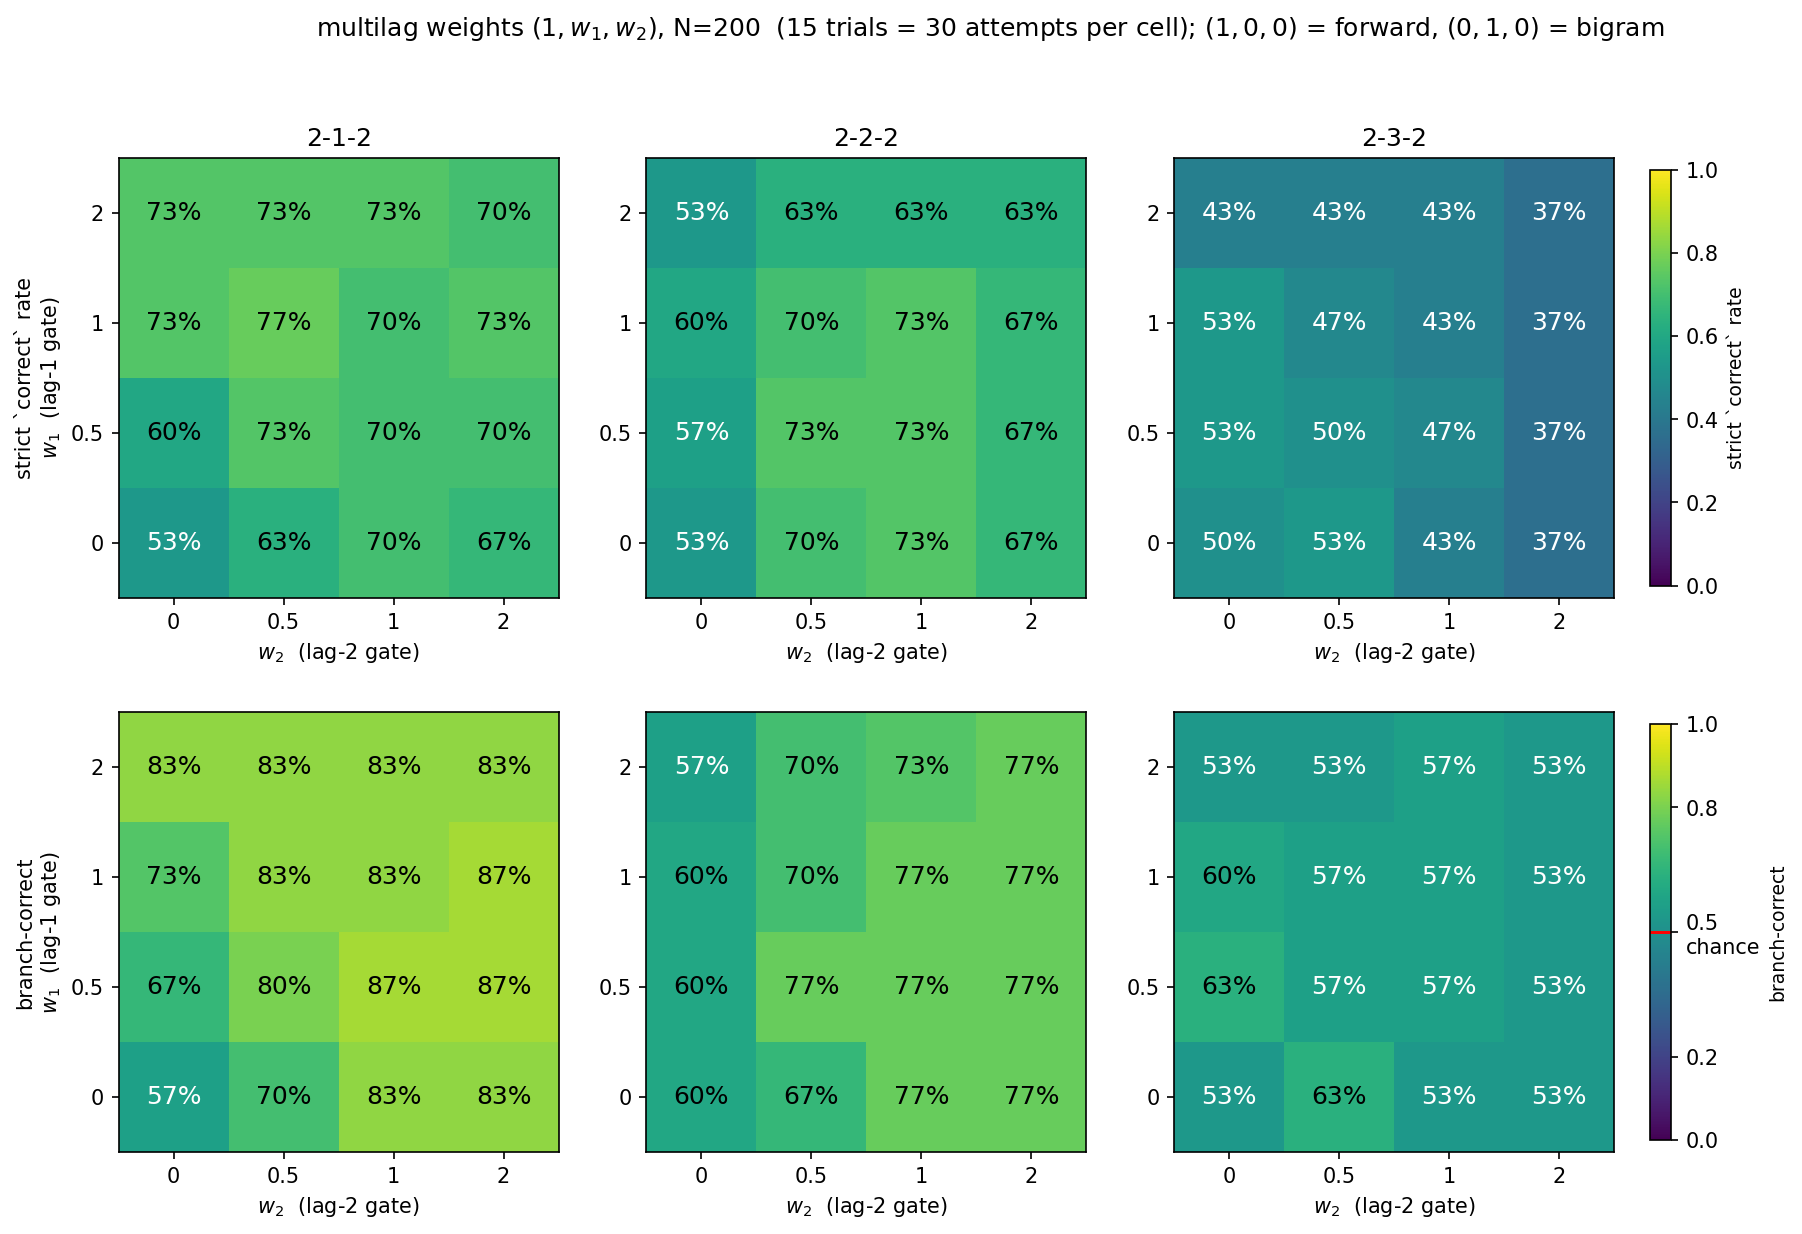
\includegraphics[width=\textwidth,height=0.50\textheight,keepaspectratio]{03_journal_club/figures/fig10_multilag_weights.png}
  \figtitle{Branch-correct rate over the multilag weights, by crossover geometry; $\omega_0$ is fixed}
  \begin{itemize}\small
    \item $\xxi^{\mu+1}\mvar_\mu\bigl(w_0\mvar_\mu^2 + w_1\mvar_{\mu-1}^2 + w_2\mvar_{\mu-2}^2\bigr)
      = w_0\,\texttt{forward} + w_1\,\texttt{bigram}_{\ell=1} + w_2\,\texttt{bigram}_{\ell=2}$:
      one rule interpolating between the catalogue entries. $w_0$ buys commitment; $w_1, w_2$ buy branch information.
    \item \textbf{\texttt{2-2-2}:} only $w_2 > 0$ lifts branch choice above chance --- reach $\ge L$, as predicted.
      \textbf{\texttt{2-3-2}:} no weighting helps.
  \end{itemize}
\end{frame}


% ---------------------------------------------------------------- 4
% [EDITED per meeting: slide 31]


\begin{frame}{4. Robustness sweep: retrieval against $N$}
  \centering
  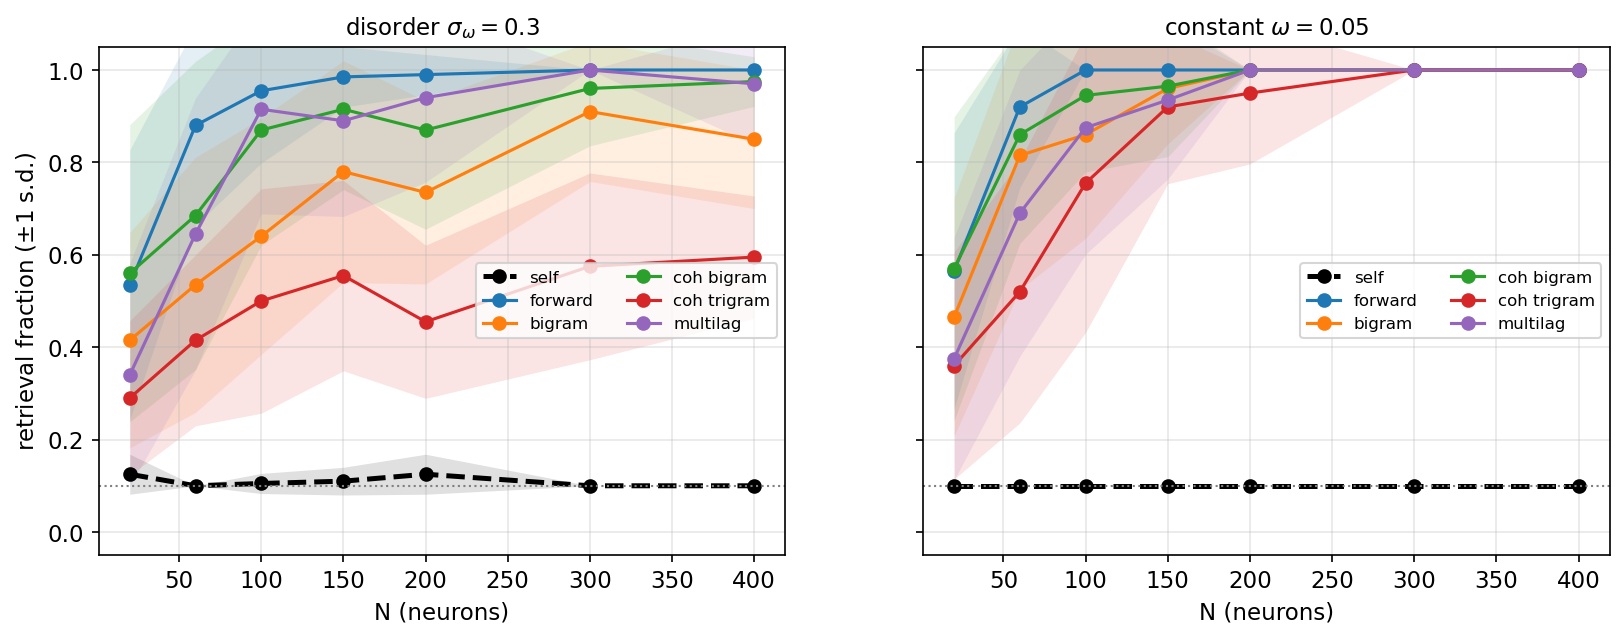
\includegraphics[width=\textwidth,height=0.4\textheight,keepaspectratio]{figures/fig07_N_sweep.png}
  \figtitle{Retrieval fraction against network size $N$ at $T = 180$, heterogeneous and constant $\omega$}
  \begin{itemize}\small
    \item Dip in performance at $N = 200$, most likely associated with scaling of the network landscape. This result contradicts with the expected behaviour of \textbf{Krotov's DAM} model. 
    \item However, as expected, \textbf{overall} retrieval \emph{improves} with $N$; more paterns are stored without crosstalk and interference.
    \item \textbf{Possible improvement:} scale the natural frequency with network size to ensure drivers traverse patterns in given simulation time.
  \end{itemize}
\end{frame}

\begin{frame}{4b. Robustness sweep: U-shaped dependence on the corruption ratio}
  \centering
  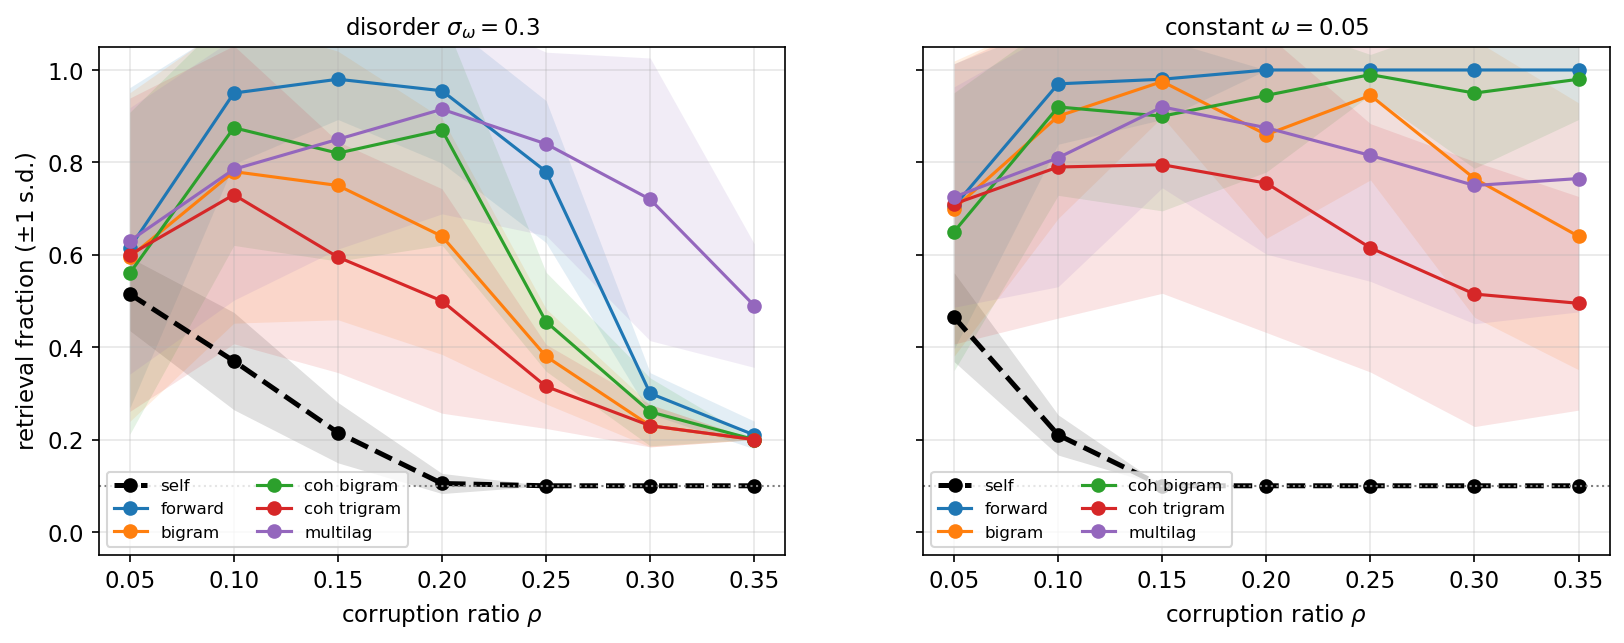
\includegraphics[width=\textwidth,height=0.42\textheight,keepaspectratio]{figures/fig08_rho_U.png}
  \figtitle{Retrieval fraction against corruption ratio $\rho$, heterogeneous and constant $\omega$}
  \begin{itemize}\small
    \item Small $\rho$: near-duplicates the
      decoder cannot separate. Large $\rho$: consecutive overlaps too small to sustain the cascade.
   
    \item \textbf{The high end is possibly regime-dependent.} Under disorder it collapses to the floor
      ($\rho = 0.35$: \texttt{forward} $0.21$, \texttt{bigram} $0.20$); at constant $\omega$ it
      barely falls (\texttt{forward} $1.00$, \texttt{coh bigram} $0.98$). The right-hand
      failure is mostly about the \emph{spread} of $\omega$.
  \end{itemize}
\end{frame}

% ---------------------------------------------------------------- findings
% [MOVED up per meeting: former slide 35; experimental conclusions]
\begin{frame}{Experimental conclusions I: learning rules}
  \begin{itemize}\small
    \item \textbf{Reach $\ge L$ only buys a chance.} The discriminating signal is a
      \emph{dynamic residual} between traversed and untraversed predecessor; it decays within
      $\sim 2$ steps. Need to account for information lost, however.
    \item \textbf{\texttt{coh trigram} is the best rule by branch choice}, the only one above
      chance at $L = 2$; \texttt{bigram}/\texttt{coh bigram} hold at $L = 1$ and fall to chance
      at $L = 2$, exactly as reach predicts; \texttt{multilag} is the most robust.
    \item \textbf{Commitment against branch information} is the governing trade-off: lagged
      factors leave fewer for self-amplification, which is why \texttt{correct} and
      \texttt{branch-correct} rank the rules differently.

  \end{itemize}
\end{frame}

% [MOVED up per meeting: former slide 36; experimental conclusions]
\begin{frame}{Experimental conclusions II: dynamics and scaling}
  \begin{itemize}\small
    \item \textbf{A natural frequency is structurally necessary.} At $\omega \equiv 0$ an exact
      cue satisfies $\sin\thetavar_i = 0$: the drive vanishes identically and the system sits at
      an exact fixed point. Either the natural frequency breaks the inherent symmetry of the memory landscapes, or is needed to alleviate integration issues with large time resolution.
    \item \textbf{Retrieval improves with $N$, like the dense memory it is built on,} and
      branch choice improves markedly with it.
      $N$ was an \emph{integration-time artifact} and is withdrawn.
    \item \textbf{U-shaped dependence on $\rho$}: interior peak. The
      high-$\rho$ collapse is mostly the \emph{spread} of $\omega$ and nearly vanishes at
      constant $\omega$; the low-$\rho$ end \emph{inflates} scores rather than depressing them; "tight packing" of patterns for low $\rho$ results in accidental retrieval of the sequence in wrong order.
   
 
  \end{itemize}
\end{frame}

% ---------------------------------------------------------------- 5

\begin{frame}[t]{Analytical claims: what is actually known?}
\small

\begin{enumerate}
\item \textbf{Coherent vs.\ magnitude gates: regime-dependent.}
\[
M_{\rm mag}\sim a\Delta |r|^2,
\qquad
M_{\rm coh}\sim a^2\Delta |r|,
\qquad
\frac{M_{\rm coh}}{M_{\rm mag}}
=\frac{a}{|r_b|+|r_c|}.
\]
Coherent reads weak residuals better; magnitude can win when predecessor
overlaps are still large.

\item \textbf{Capacity is slot-counting.}
\[
\mathbb{E} |A|^2=\frac{\kappa}{N^n},
\qquad
P_{\max}\sim \frac{S^2}{\kappa}N^n,
\qquad
\kappa=\prod_i k_i! .
\]
Repeated slots only change the prefactor; order changes the exponent.

\item \textbf{Context weights should grow with lag.}
If \(|r_k|\simeq\lambda^k|r_0|\), equalising lag strength suggests
\[
w_k\propto\lambda^{-pk},
\qquad
p=2\ \text{magnitude},\quad p=1\ \text{coherent}.
\]
The scale \(w_2/w_1\approx2\) is supported, but not yet a unique optimum.
\end{enumerate}

\end{frame}

% [EDITED per meeting: slide 34]
\begin{frame}{Outlook: open questions}
  \centering
  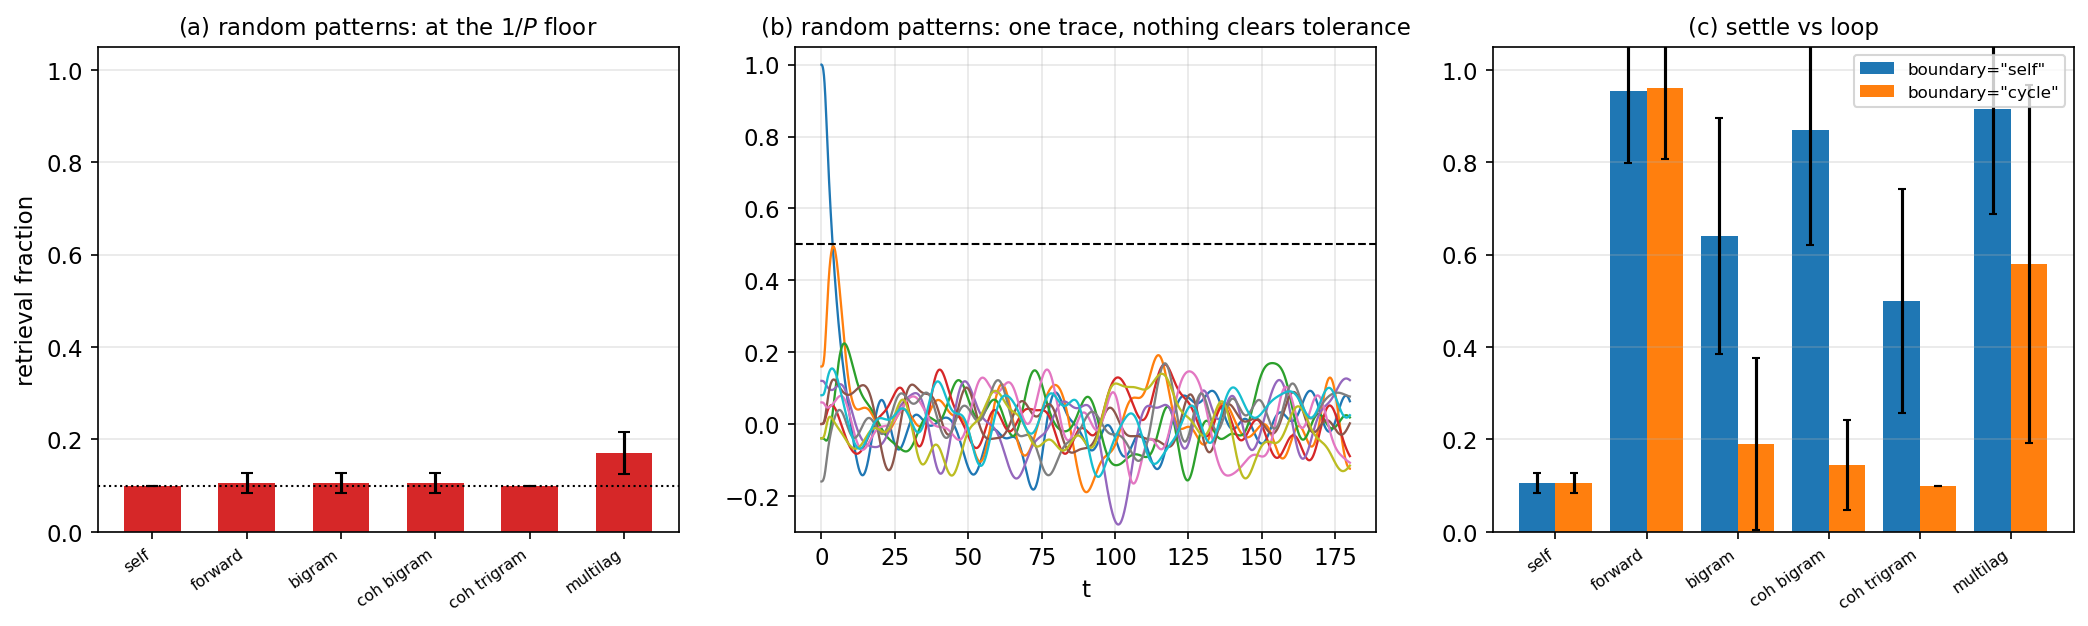
\includegraphics[width=\textwidth,height=0.36\textheight,keepaspectratio]{figures/fig09_appendix.png}
  \figtitle{Controls: independently random patterns (a,b) and \texttt{boundary="cycle"} (c)}
  \begin{itemize}\small
    \item \textbf{Random patterns:} worst case, but analytically tractable.
    \item \textbf{Effect of noise.} (Euler–Maruyama or Network at Temperature)
    \item \textbf{(a,b) Random patterns.} Replace the mutation chain with independently random
      patterns and retrieval disappears for \emph{every} rule --- all at the $1/P$ floor, with
      peak overlaps far below \texttt{tolerance}. Sequential similarity structure is a
      prerequisite.
    \item \textbf{(c) \texttt{boundary="cycle"} does not work.} Settling is what makes each
      pattern a usable attractor long enough to be decoded. Wiring the
      last pattern back to the first removes the terminal fixed point and the trajectory
      degrades rather than looping.
  \end{itemize}
\end{frame}



\section[Analysis]{Theoretical Analysis}

% [NEW] learning rule in tensor form; symmetric / asymmetric split; analytical setting
\begin{frame}{Rough Draft for Theoretical analysis: learning rule in tensor form}
  \small
  \[
    \dot{\boldsymbol{\thetavar}} = \boldsymbol{\omega} - \sin\boldsymbol{\thetavar} \odot
      \boldsymbol{\Xi}^{\top}\,\mathbf{J}\bigl[\mathbf{m}^{\otimes d}\bigr],
    \qquad
    \mathbf{m} = \tfrac{1}{N}\,\boldsymbol{\Xi}\cos\boldsymbol{\thetavar},
    \qquad
    \mathbf{J} = \mathbf{J}^{\mathrm{S}} + \mathbf{J}^{\mathrm{A}}
  \]
  {\footnotesize $\boldsymbol{\Xi} \in \{-1,+1\}^{P\times N}$: stored patterns;
  $\mathbf{m} \in \mathbb{R}^{P}$: overlaps (leave-one-out in simulation);
  $\mathbf{J}$: rank-$(d{+}1)$ transition tensor built from the rule table.}
  \vspace{2mm}
  \begin{columns}[T]
    \begin{column}{0.48\textwidth}
      \begin{block}{Symmetric component $\mathbf{J}^{\mathrm{S}}$}
        \footnotesize
        Retrieval of the current pattern; stabilises the dynamics. 
      \end{block}
    \end{column}
    \begin{column}{0.48\textwidth}
      \begin{block}{Asymmetric component $\mathbf{J}^{\mathrm{A}}$}
        \footnotesize
        Drives transitions; lag-context terms \textbf{alleviate branch ambiguity.}
      \end{block}
    \end{column}
  \end{columns}
  \vspace{2mm}
  {\footnotesize Inspired by Katahira et al., arXiv:cond-mat/0702427 (2007);
  Kawamura \& Okada, J.\ Phys.\ A \textbf{35}, 253 (2002).}
  \vspace{2mm}
  \begin{block}{Analytical setting: random rather than smooth patterns}
    \footnotesize
    (i) Worst case: uncorrelated patterns yield the $1/P$ floor numerically for every rule.
    (ii) For i.i.d.\ patterns the crosstalk statistics are tractable, so scaling in $N$ and $P$
    can be treated analytically. 
  \end{block}
\end{frame}
\section[Conclusions]{Conclusions and Outlook}
% =====================================================================



\begin{frame}{Conclusions}
  \begin{block}{Main result}
    To resolve branching after a shared segment, the learning rule needs a
    \textbf{lag reference exceeding the length of the shared segment.} Only a
    factor reading back past the last shared pattern breaks the innate
    symmetry of the Lyapunov function; rules whose lags all sit inside the
    shared run are symmetric in the branches by construction.
  \end{block}
  \begin{itemize}
    \item Sufficient reach is only the entry ticket: commitment and
      branch information trade off.
    \item The rule alone does not fix the operating point: $\rho$, $N$ and
      $\sigma_\omega$ provide necessary conditions for a smooth retrieval.
  \end{itemize}
\end{frame}


% =====================================================================
\section[Open Questions]{Active Questions for Further Investigation}
% =====================================================================

\begin{frame}{Active questions}
  \begin{enumerate}
    \item Effect of boundary conditions on short sequences: verifying whether decay of lag-based learning rules is alleviated by extending sequences.
    \item With greater computing power, increase temporal resolution and attempt $\omega=0$ sequence retrieval.
    \item How are these learning rules implemented in \textbf{physical
      (oscillator-based) simulators}?
    \item What is the role of \textbf{decaying neurons}, and can they
      replace the explicit lag buffer?
    \item How does one generate \textbf{robust rules for randomly generated
      pattern sequences}?
    \item overlap of M+ sequences.
  \end{enumerate}
  \vspace{3mm}
  {\small Further open questions: whether the resolvable shared-run length
  $L$ admits a fundamental ceiling, and whether rule weights can be
  \emph{learned} rather than constructed by hand.}
\end{frame}

\begin{frame}
  \centering
  \Large Thank you \\[2mm]
  \small \textbf{https://github.com/dvnrlv/Kuramoto-CD-DAM}
  \begin{figure}
      \centering
      
\includegraphics[width=0.5\linewidth]{03_journal_club/figures/github.png}
      \caption{Caption}
      \label{fig:placeholder}
  \end{figure}
\end{frame}


% =====================================================================
% [NEW per meeting] appendix
% =====================================================================
\appendix
\section*{Appendix}

% [MOVED to appendix per meeting: former slide 11]
\begin{frame}{Objects: patterns, overlaps, couplings}
  \centering
  \small
  \begin{tabular}{lll}
    \toprule
    Object & Shape & Content \\
    \midrule
    $\thetavar$            & $N$         & oscillator phases; $s_i = \cos\thetavar_i$ \\
    $\xxi^{a,\mu}$         & $K \times P \times N$ & stored patterns,
      $\xxi_i = \cos\varphi_i \in \{-1,+1\}$, $\varphi_i \in \{0,\pi\}$ \\
    $\xxi^{a,\mu+1}$       & $K \times P \times N$ & successor tensor: row $\mu$ holds
      the pattern $\mu$ drives \\
    $\mvar_i^{a,\mu}$      & $K \times P$ (per $i$) & leave-one-out overlaps,
      $\frac{1}{N-1}\sum_{j \ne i}\xxi_j^{a,\mu}\cos\thetavar_j$ \\
    $T^a_{\alpha\beta}$    & $K \times P \times P$ & transition matrix; row $=$
      destination, column $=$ source \\
    $R$ (rule table)       & $n_{\text{terms}} \times (d+2)$ &
      rows $[\,s \mid \ell_1 \dots \ell_d \mid w\,]$: target offset, lags, weight \\
    $J$ (coupling)         & rank $d+1$  & $J_i^{\mu_1 \dots \mu_d,\,\nu}$, contracted
      against $d$ overlaps \\
    \bottomrule
  \end{tabular}
  \\[3mm]
  \begin{itemize}
    \item Patterns are real, so $|\mvar|^2 = \mvar^2$: the write-up's fourth-order
      bidegree-$(2,1)$ fields are the $d = 3$ rows of $R$.
    \item $T$ sums \emph{pure powers} $\sum_\beta T_{\alpha\beta}(\mvar^\beta)^d$;
      a rule table multiplies overlaps read at \emph{different} lags, which no $T$ can
      express. The shift matrix $T_{\alpha\beta} = \delta_{\alpha,\beta+1}$ and the row
      $[\,1 \mid 0,0,0 \mid 1\,]$ are the same baseline.
  \end{itemize}
\end{frame}

\end{document}